
\documentclass{article} % For LaTeX2e
\usepackage{iclr2027_conference,times}

% Optional math commands from https://github.com/goodfeli/dlbook_notation.
% math_commands.tex redefines eqref to print "equation N", so the text cites equations as Eq. (N).
\input{math_commands.tex}

\usepackage{hyperref}
\usepackage{url}
\usepackage{amsmath,amssymb,amsthm}
\usepackage{graphicx}
\usepackage{booktabs}
\usepackage[table]{xcolor}



\definecolor{cPos}{RGB}{58,164,110}
\definecolor{cNeg}{RGB}{217,106,89}
\definecolor{stdgray}{gray}{0.45}

% Shading in results tables marks only the cells a table's claim rests on,
% in \cellcolor{cPos!60}; every other cell is unshaded, and each caption says
% what its shaded cells show.

\newtheorem{definition}{Definition}
\newtheorem{proposition}{Proposition}

\title{Stale, Misattributed, or Late: What Personal Fact Retrieval Puts in the Prompt}

% Authors must not appear in the submitted version. They should be hidden
% as long as the \iclrfinalcopy macro remains commented out below.
\author{Anonymous authors}

%\iclrfinalcopy % Uncomment for camera-ready version, but NOT for submission.
\begin{document}

\maketitle

\begin{abstract}
A language assistant that uses remembered personal facts can fail in three ways that one accuracy number cannot separate: the prompt can carry a value that has since been revised, a value belonging to a different person of the same name, or nothing at all because retrieval finished after generation began. We formalize these as stale exposure, misattribution and lateness and score them on the prompt rather than the answer, including on requests the store cannot answer, which a product of recall terms zeroes. Scored there they come apart: each is decided in a different place and yields to a different fix. Staleness is settled at write time by a rule several memory systems implement --- key a fact to its subject and property, serve only the open value --- which we adopt unchanged, claim no novelty for, and price. Given correct keys it removes stale exposure for every retriever we tried and the ranker stops mattering: the premise, not the ledger, is the expensive part. Its two failure modes are not symmetric --- a missed merge leaves an extra line in the prompt, a false merge deletes a value silently --- and that inverts the usual reading of an extractor. Four models from 3B to 14B beat a rule extractor on key recall, 0.980 to 0.996 against 0.807, and every one leaves a dirtier prompt, 0.560 to 0.644 against 0.781; on LongMemEval, where keys must be discovered from open text, the mechanism never fires, even shown the keys already in the store. The other two failures are decided on the serving path and survive all of it. A posterior over the entities a name could denote cuts wrong-person exposure from 0.121 to 0.032 at no recall cost, where filtering on the interlocutor costs 98\% of facts about third parties; neither helps on LoCoMo, where two speakers are one string. Nothing abstains unless a gate is added, and the gate that works needs a slot inventory the open corpora lack. The block itself then costs three orders of magnitude more than the retrieval that filled it.
\end{abstract}

\section{Introduction}

A user drafts a message to a colleague, Alex Chen, and the assistant offers a continuation of ``the standup with Alex is at''. A useful continuation carries the time the two of them last agreed on. Three things can go wrong in the memory layer before the model writes a word: the prompt can hold 9:30am after the meeting moved to 10:45am, it can hold the time agreed with a different Alex, or the lookup can still be running when prefill starts. We call these staleness, misattribution and lateness.

Several memory systems handle the first at write time, keying a fact by its subject and the property it states, closing the old value when a new one arrives, and retrieving only what is open~\citep{rasmussen2025zep,chhikara2025mem0,yadav2026memstrata,wang2026toki}; they report that stale answers all but disappear. The rule is standard in temporal databases~\citep{jensen1999temporal} and we adopt it unchanged; our question is what it is worth, and what it leaves untouched, measured on the object the model actually reads. That object is the prompt, which current evaluations do not score: LoCoMo, LongMemEval, MemoryAgentBench and Memora score the answer~\citep{maharana2024evaluating,wu2024longmemeval,hu2026memoryagentbench,uddin2026memora}, and even a forgetting-aware score cannot see a prompt that held the current value and a superseded one at once and got lucky. We record instead, per request, whether the injected block holds the current value, a superseded value of the same slot, a same-named other person's value, or nothing at all, and how long it took to produce.

Measured there, the write-time rule looks different. Given correct keys it removes stale exposure for every retriever we tried, so the ranker barely matters; but the keys have to come from somewhere, and the two ways of getting them wrong are not symmetric. A missed merge leaves an extra line in the prompt; a false merge deletes a correct value, silently. That is enough to put every model we tried, from 3B to 14B and all above 0.980 key recall, behind a rule extractor at 0.807, and on LongMemEval the mechanism does not fire at all. The other two failures are untouched: wrong-person exposure survives every ranker and validity filter, and a retriever with a fixed $k$ cannot report that it found nothing.

We contribute (i) a prompt-level decomposition and its metrics, with a two-case definition that scores requests the store cannot answer (Eq.~\ref{eq:clean}) rather than zeroing them; (ii) a measurement of what write-time validity is worth, breaking its premises one at a time through key noise at known rates, key granularity, out-of-order arrival, a ladder of four models assigning keys on paraphrased text, and open-domain key discovery; (iii) two serving-side rules for the failures it does not cover, each reported with the recall it costs and the corpus on which it stops working; and (iv) latency accounting, including a waiting bound whose assumptions we measure on the path it bounds. Everything runs on synthetic corpora we control and two public ones we did not, with two-level bootstrap intervals, cluster-level permutation tests and equivalence tests wherever we call two arms interchangeable.

\section{Related Work}

\paragraph{Write-time validity, and why we claim none of it.}\label{sec:related_validity}
Agent memories score observations by recency and relevance~\citep{park2023generative}, add forgetting curves~\citep{zhong2024memorybank}, page between tiers~\citep{packer2023memgpt}, link atomic notes~\citep{xu2025amem}, or retrieve over entity graphs and abstractions~\citep{gutierrez2024hipporag,xia2026memora}. A subset decides at write time which version is current and serves only that one, whether by a model judging contradiction~\citep{rasmussen2025zep,chhikara2025mem0} or by a deterministic rule over (subject, relation, object) triples in a bi-temporal ledger~\citep{yadav2026memstrata,wang2026toki}; others resolve conflicts at read time~\citep{banerjee2026apex} or reorder on stated rather than dialogue time~\citep{su2026beyond}.

Our rule is MemStrata's, one key shape away, and Proposition~\ref{prop:one_active} is the state invariant any of these designs maintains, itself standard for transaction-time databases~\citep{jensen1999temporal}. We claim no novelty for it, and use it because this paper's question is the one those results leave open: MemStrata reports stale-fact errors falling from 15--40\% to about zero and TOKI's theorems hold by construction, but both presuppose that an update was recognized as one and attached to the right key. Sections~\ref{sec:keynoise} and~\ref{sec:real} ask what happens when it was not.

\paragraph{What the prompt hides that the answer does not.} Evaluations of agent memory mostly score the final answer: LoCoMo and LongMemEval over long histories~\citep{maharana2024evaluating,wu2024longmemeval}, MemoryAgentBench with selective forgetting as a competency~\citep{hu2026memoryagentbench}, Memora with an accuracy penalizing reliance on invalidated memory~\citep{uddin2026memora}, MemConflict with conflicts built on purpose~\citep{tao2026memconflict}, and STALE by asking whether a model notices its own memory has expired~\citep{chao2026stale}; closest to us, MemTrace probes the retrieved context as well as the answer~\citep{long2026memtrace}. We differ in what is scored and what is controlled. An answer-level score, forgetting-aware or not, is one number over a prompt that may hold the current value, a superseded value and a third person's value at once: Table~\ref{tab:temporal} shows a store with 0.950 current-value recall and 0.703 stale exposure, which no answer-level metric distinguishes from a clean one. MemTrace keeps retrieval and generation as its stages; we cut along failure modes instead, because the three turn out to be decided in different places. STALE and MemConflict ask whether a system handles a conflict; we ask what reaches the prompt before the model is consulted, and add two failures neither covers: a name that denotes the wrong person, and a request answered after generation began. None of this work prices the memory block, which Section~\ref{sec:llm} finds costs three orders of magnitude more than the retrieval that filled it; work on memory cost~\citep{zhao2025ame,yuan2026agentir,zhou2026we} and lock-free publication~\citep{mckenney1998rcu,mccandless2010lucene} informs our serving path.

\section{Problem Formulation}
\label{sec:problem}

Requests are indexed by $t$ and arrive at $\tau_t$; $\mathcal{M}_t$ is the set of facts retained then, history included. A request carries local context $c_t$, a participant set $P_t$, a fact limit $k$, a character budget $B$ and a deadline $D_t$.

\begin{definition}[Personal fact]
A stored fact is $f=(z_f,E_f,P_f,\kappa_f,a_f,b_f,s_f)$: prompt-ready text, normalized entities, the participants of the source observation, an optional key naming a mutable slot, the interval $[a_f,b_f)$ during which the store treats $f$ as active ($b_f=\infty$ until $f$ is superseded), and the time $f$ was last observed. The active view is $\mathcal{A}_t=\{f\in\mathcal{M}_t:a_f\le\tau_t<b_f\}$.
\end{definition}

That interval records the store's state, not the truth: an extractor that misses a revision leaves an outdated fact active. A policy $\pi$ maps $(\mathcal{M}_t,c_t,P_t)$ to an ordered $S_{\pi,t}\subseteq\mathcal{M}_t$ in time $L_{\pi,t}$, subject to $|S_{\pi,t}|\le k$ and a serialized length of at most $B$; it may restrict itself to $\mathcal{A}_t$ or ignore the intervals, so validity-agnostic retrievers are admissible. $R_t(f)=1$ when $f$ states a value for the slot asked about, for any entity whose name matches the surface form used, so $R_t$ ignores identity; $I_t(f)=1$ when $f$ concerns the intended entity; $V_t(f)=1$ when its value is still current. The target set is $\mathcal{G}_t=\{f:R_t(f)=I_t(f)=V_t(f)=1\}$, and the policy sees none of these labels. Current-value recall is $C_{\pi,t}=\mathbf{1}\{S_{\pi,t}\cap\mathcal{G}_t\neq\varnothing\}$, stale exposure is $E^{\mathrm{stale}}_{\pi,t}=\mathbf{1}\{\exists f\in S_{\pi,t}:R_t(f)=I_t(f)=1,V_t(f)=0\}$, and misattribution is $E^{\mathrm{id}}_{\pi,t}=\mathbf{1}\{\exists f\in S_{\pi,t}:R_t(f)=1,I_t(f)=0\}$. With $\mathcal{G}_t=\varnothing$ there is nothing to recall, so $C_{\pi,t}$ is zero for every policy including a correct one, and a product of the three indicators scores a correct abstention and a confident wrong answer alike. The prompt is therefore clean in two cases,
\begin{equation}
Y_{\pi,t}=
\begin{cases}
C_{\pi,t}\,(1-E^{\mathrm{stale}}_{\pi,t})(1-E^{\mathrm{id}}_{\pi,t}), & \mathcal{G}_t\neq\varnothing,\\[2pt]
1-\mathbf{1}\{\exists f\in S_{\pi,t}:R_t(f)=1\}, & \mathcal{G}_t=\varnothing,
\end{cases}
\qquad Y_{\pi,t}(D)=Y_{\pi,t}\,\mathbf{1}\{L_{\pi,t}\le D\},
\label{eq:clean}
\end{equation}
which we report separately and never pool, since a policy that abstains often scores well on the second at the expense of the first. We also record the abstention rate $A_{\pi,t}=\mathbf{1}\{S_{\pi,t}=\varnothing\}$: a fixed-$k$ retriever has $A_{\pi,t}=0$ by construction. The indicators are not exclusive, so a prompt can hold the current value and a superseded one at once, which recall alone hides.

Suppose now that every recognized revision of a slot carries the same key $\kappa$ and updates are applied in receipt order, so that committing $f'$ with key $\kappa$ at $u$ sets $a_{f'}=u$, $b_{f'}=\infty$ and $b_f=u$ for the active predecessor, which stays as history, atomically for readers.

\begin{proposition}[At most one active value per key]
\label{prop:one_active}
Fix a key $\kappa$. If updates carrying $\kappa$ are committed serially and atomically by the rule above, and at most one fact with key $\kappa$ is active initially, then every reader-visible state satisfies $|\{f\in\mathcal{A}:\kappa_f=\kappa\}|\le 1$.
\end{proposition}

The proof is in Appendix~\ref{app:proofs}. The statement is narrow and says nothing about whether the surviving value is right; under out-of-order arrival the last to arrive stays active, not the last stated. Two extractor errors break it in opposite ways: a \emph{missed merge} gives two revisions different keys, so both stay active, and a \emph{false merge} gives one entity's revision another entity's key, so that entity loses its current value.

\section{A Reference Memory Layer}
\label{sec:pfm}

To measure what enters the prompt we need a layer whose every stage is logged and whose parameters are fixed in advance. We use Personal Fact Memory (PFM), which implements the keyed-supersession rule of Section~\ref{sec:related_validity} with the update decision made by a key comparison at commit time rather than by a model call. Nothing here is a new mechanism; Appendix~\ref{app:config} gives every formula and constant.

An extractor turns an observation into drafts with text, entities and an optional slot key. On the controlled benchmark a rule keys a sentence naming a gazetteer entity, a slot noun and a value of that slot's type; the public corpora of Section~\ref{sec:real} have neither, so there the drafts are plain sentences and the key comes from a model. A keyed draft repeating the active value of its key is a re-observation; any other supersedes it. A keyless draft is absorbed only when an active fact sharing an entity has token Jaccard at least $0.8$ \emph{and} the same value-bearing tokens --- without that second condition, ``the standup with Alex is moved to 9:30am'' absorbs ``\ldots moved to 10:45am'' and the revision is lost although no key was involved. Superseded facts leave the index and stay as history, and pruning exempts the active fact of every key. Serving scores active facts by simple BM25F~\citep{robertson2004simple,robertson2009probabilistic} over text, entity and participant fields, times recency and usage factors, plus a one-hop graph term, then takes facts in score order until $k$ or $B$ would be exceeded; no embedding and no language model runs on this path. A background worker also publishes immutable snapshots a request can read instead of waiting, which Appendix~\ref{app:serving} bounds (Proposition~\ref{prop:waiting}) conditional on a hand-off cost and a scheduling delay we measure rather than assume.

\section{Identity and Abstention on the Serving Path}
\label{sec:identity}

Supersession decides which value of a slot is current. It says nothing about which entity the request is about, or whether the store has that entity's value at all, and no ranker we tried does either. Both are decisions on the ranked list, and both can be made without a model call.

A name token of the request is a \emph{mention}, ambiguous when several stored entities answer to it, as a first name does; tokens that pick out one entity are left alone. For the candidate set $\mathcal{E}_t$ of an ambiguous mention we score each $e$ and take a posterior:
\begin{equation}
\psi_t(e)=w_p\,\mathbf{1}\{e\in P_t\}+w_g\!\!\sum_{p\in P_t}\!\frac{w_{pe}(\tau_t)}{\sum_v w_{pv}(\tau_t)}+w_r\,2^{-(\tau_t-s_e)/T_{\mathrm{rec}}},
\qquad
\pi_t(e)=\frac{e^{\psi_t(e)/T}}{\sum_{e'\in\mathcal{E}_t}e^{\psi_t(e')/T}},
\label{eq:identity}
\end{equation}
where $s_e$ is the most recent active fact about $e$, $w=(1,1,0.25)$ and $T=0.5$: the candidate is the interlocutor, the graph links it to the interlocutor, the store saw it recently. Retrieval keeps facts about $\arg\max_e\pi_t(e)$ and facts about no candidate. The middle term is what separates this from filtering on the conversation: a hard participant filter is the special case putting all mass on $P_t$, which removes wrong-person exposure on a benchmark whose facts are about the person one is talking to and deletes almost everything about third parties, whereas the graph term requires only that the subject has been discussed with the interlocutor.

A block that states nothing is the correct block when the store holds nothing. The \emph{slot gate} recognizes the slot a request asks for from its noun and trailing cue and returns nothing unless some retrieved fact states that slot for a candidate with $\pi_t(e)\ge\tau$. The \emph{margin gate} needs no slot inventory: it returns nothing unless the top fact scores at least $\tau$ times the shortlist mean and shares a third of the request's content terms. The first is the stronger rule and the narrower one, so we report both on both kinds of corpus (Appendix~\ref{app:identity}).

\section{Experimental Setup}
\label{sec:setup}

\paragraph{Corpora.} The controlled benchmark builds 160 revision chains per instance over (entity, slot) pairs from 36 people, 20 projects and six slot types, with zero to four revisions each and 1{,}000 filler messages. Queries are message prefixes such as ``Just confirming, Alex standup is now at'', carrying the chain's participant as $P_t$ and naming people by first name, so a chain on the same slot whose person shares that first name is a wrong-person competitor: 40--50 of the 240 queries per instance are ambiguous this way. Five instances give 1{,}200 queries, and values unique within an instance make exposure a whole-token containment check. Two public corpora remove what the generator supplies. \emph{LongMemEval}~\citep{wu2024longmemeval} carries staleness: its 78 knowledge-update questions each annotate two answer-bearing user turns, an earlier one stating a value later revised and a later one stating the value in force, which a local model turns into exact labels by copying the verbatim span of each; it has no slot vocabulary, so keys must be discovered. \emph{LoCoMo}~\citep{maharana2024evaluating} carries misattribution, because the name John belongs to a speaker in three of its ten conversations, so over one store built from all ten a block answering a question about one John with a fact from another's conversation is a misattribution by provenance; per-conversation stores supply unanswerable requests (Appendices~\ref{app:bench},~\ref{app:real}).

\paragraph{Arms and statistics.} Every arm ranks facts from the same store through the same greedy selection and block format with $k=6$ and $B=800$ ($B=1200$ on the public corpora). BM25 uses text only; ``+ validity'' restricts an arm to the active facts PFM serves; ``+$P_t$'' appends participant names to the query and to each fact's text; Dense is all-MiniLM-L6-v2, and Hybrid fuses both shortlists by reciprocal rank. Queries of one chain share a label set and chains of one instance share a seed, so intervals come from a two-level bootstrap over seeds then chains, and a rate of 0 or 1 gets the Wilson interval over the number of \emph{chains} with an event, so 0 of 800 reads as a bound. Paired comparisons use a permutation test that flips the sign of a whole chain at a time, since McNemar treats one chain's queries as independent. A difference that fails to reach significance is not equivalence, so where we call two arms interchangeable we run two one-sided tests against a margin fixed in advance at $\pm0.02$ clean retrieval~\citep{schuirmann1987tost}.

\section{Results}

\subsection{Supersession, and What the Ranker Adds}
\label{sec:temporal}

\begin{table}[t]
\centering
\small
\setlength{\tabcolsep}{3pt}
\begin{tabular}{@{}llrrrrr@{}}
\toprule
Store & $B$ & Current $\uparrow$ & Stale $\downarrow$ & Wrong-person $\downarrow$ & Co-injection $\downarrow$ & Clean $\uparrow$ \\
\midrule
Keyed & 800 & 0.998 {\scriptsize(0.993, 1.000)} & \cellcolor{cPos!60}0.000 {\scriptsize(0.000, 0.005)} & 0.121 {\scriptsize(0.094, 0.149)} & 0.000 {\scriptsize(0.000, 0.005)} & \cellcolor{cPos!60}0.877 {\scriptsize(0.850, 0.904)} \\
Keyless & 800 & 0.950 {\scriptsize(0.923, 0.971)} & 0.703 {\scriptsize(0.654, 0.749)} & 0.004 {\scriptsize(0.000, 0.012)} & 0.701 {\scriptsize(0.652, 0.746)} & 0.247 {\scriptsize(0.210, 0.284)} \\
\midrule
Keyed & 240 & 0.869 {\scriptsize(0.836, 0.903)} & 0.000 {\scriptsize(0.000, 0.005)} & 0.000 {\scriptsize(0.000, 0.005)} & 0.000 {\scriptsize(0.000, 0.005)} & 0.869 {\scriptsize(0.836, 0.903)} \\
Keyless & 240 & 0.823 {\scriptsize(0.791, 0.852)} & 0.446 {\scriptsize(0.396, 0.501)} & 0.000 {\scriptsize(0.000, 0.005)} & 0.438 {\scriptsize(0.388, 0.493)} & 0.385 {\scriptsize(0.331, 0.435)} \\
\bottomrule
\end{tabular}
\caption{Keys remove stale values from the prompt. Each entry is the share of 1{,}200 queries whose memory block --- what enters the prompt, not the model's answer --- holds the \emph{current} value, a since-revised \emph{stale} one, a same-named \emph{wrong person}'s, current and stale together (\emph{co-injection}), or the current value and neither error (\emph{clean}). $\uparrow$/$\downarrow$: higher/lower is better; columns overlap, so rows need not sum to one. $B$: characters in the block. Parentheses: 95\% intervals; an exact 0 takes the Wilson bound over 800 chains, so 0.000 (0.000, 0.005) means at most 0.5\%. Shaded: the cells that claim rests on. Keyless blocks show few wrong-person values only because stale ones fill them.}
\label{tab:temporal}
\end{table}

\begin{table}[t]
\centering
\small
\setlength{\tabcolsep}{4pt}
\begin{tabular}{@{}lrrrrrr@{}}
\toprule
Method & Current $\uparrow$ & Stale $\downarrow$ & Wrong-person $\downarrow$ & Clean $\uparrow$ & p50 (ms) $\downarrow$ & p99 (ms) $\downarrow$ \\
\midrule
PFM & 0.998 & 0.000 & 0.121 & \cellcolor{cPos!60}0.877 {\scriptsize(0.850, 0.904)} & 0.25 & 0.69 \\
BM25 + validity & 0.891 & 0.000 & 0.120 & 0.774 {\scriptsize(0.737, 0.809)} & 0.09 & 0.26 \\
BM25 + validity + $P_t$ & 1.000 & 0.000 & 0.128 & \cellcolor{cPos!60}0.873 {\scriptsize(0.847, 0.896)} & 0.10 & 0.29 \\
Dense + validity + $P_t$ & 1.000 & 0.000 & 0.164 & 0.836 {\scriptsize(0.803, 0.868)} & 18.3 & 93.0 \\
Hybrid + validity + $P_t$ & 1.000 & 0.000 & 0.157 & 0.843 {\scriptsize(0.813, 0.872)} & 18.2 & 82.4 \\
\midrule
BM25 + $P_t$ (no validity) & 0.997 & 0.802 & 0.007 & 0.195 {\scriptsize(0.164, 0.227)} & 0.18 & 0.46 \\
\bottomrule
\end{tabular}
\caption{With validity, the ranker barely matters. Columns as in Table~\ref{tab:temporal}; same stores, $k{=}6$, $B{=}800$. \emph{+ validity}: superseded facts cannot be retrieved; \emph{+ $P_t$}: participant names join the query and each fact. Last row: the best arm without validity (all eight in Appendix~\ref{app:full}). p50/p99: median/99th-percentile retrieval latency. Shaded: equivalent within $\pm0.02$.}
\label{tab:baselines}
\end{table}

The keyed and keyless stores receive identical drafts; the keyless store ignores keys. Supersession removes stale exposure: none of 1{,}200 keyed prompts over 800 chains holds a superseded value (a rate of at most 0.005), while 70.3\% of keyless prompts do, almost always beside the current value. The benchmark revises 80\% of its chains, more than a personal store is likely to; reweighting to 70\% never revised lifts the keyless store to 0.603 and leaves the ordering unchanged (Table~\ref{tab:depth}). The keyed store's remaining errors are all wrong-person exposures on ambiguous queries, and in 94 of the 145 the correct fact ranks first while a competitor fills a later slot --- so Section~\ref{sec:idresults} treats identity as a decision about the whole block, not the top rank.

\emph{Validity comes from the store, not the ranker.} Every arm restricted to active facts has zero stale exposure, and every arm without that restriction exposes a stale value on 78--80\% of queries once it receives $P_t$; dense retrieval recalls the current value almost always yet has the highest stale exposure, because every version of a revised fact is equally similar to the query. Once the store and the participant are shared the ranker barely matters: BM25 + validity + $P_t$ reaches 0.873 clean against PFM's 0.877, a paired difference of 0.005 with a 90\% interval of $-$0.008 to 0.019, inside the $\pm0.02$ margin fixed in advance, so the two are equivalent at that margin ($p_{\mathrm{TOST}}=0.038$), which a permutation test alone ($p=0.55$) could not show. Without $P_t$ the same arm drops to 0.774 and PFM leads by 0.103 (CI 0.082 to 0.127), so the participant name accounts for the gap; an ablation agrees: dropping the participant signals costs up to 0.122 clean retrieval, while the entity field, graph, usage term, recency and term cap change nothing (Table~\ref{tab:ablation}). What these results support is an active-only store plus participant-aware lexical retrieval, not the rest of Section~\ref{sec:pfm}. Dense and hybrid with validity are worse rather than equivalent, by 0.042 (CI 0.025 to 0.059) and 0.034 (CI 0.018 to 0.050), through wrong-person exposure and not recall; and they clear a 10~ms deadline almost never, because MiniLM query encoding alone costs 18~ms at the median (Figure~\ref{fig:deadline}).

\subsection{What the Keys Are Worth}
\label{sec:keynoise}


Proposition~\ref{prop:one_active} assumes revisions of a slot share a key, so we corrupt keys after extraction. Stale exposure grows almost in proportion to the missed-merge rate $p$ --- 0.100 at $p{=}0.05$, 0.370 at $0.2$, 0.592 at $0.4$, approaching the keyless store's 0.703 --- and is visible in the prompt. False merges fail silently instead: at $q{=}0.05$, 6.1\% of queries have lost their current value from the active view; at $q{=}0.2$, 22.5\% have and clean retrieval falls to 0.553 (Table~\ref{tab:keynoise}). Key granularity and arrival order matter for the same reason: a key at (entity, slot) merges a person's standup with their sync and drops current-value recall to 0.500, and delivering 30\% of chains out of order costs 0.130, which ordering by stated time repairs exactly (Appendix~\ref{app:slices}).

\paragraph{Keys from a model.}\label{sec:extractor}
One model (qwen2:7b, greedy) rewrites every chain message of three corpora in its own words, keeping names and values; 1{,}012 of 1{,}268 rewrites are accepted and the rest fall back to the template. The rewriter is held fixed, so every key assigner reads the same text. We compare the rule extractor of Section~\ref{sec:pfm}; the same pipeline with keys from four models spanning 3B to 14B and two generations; a model-resolved path choosing ADD, UPDATE, DELETE or NOOP over the five most similar active facts, the shape of Mem0's update decision~\citep{chhikara2025mem0} in our implementation; and no update resolution at all.

\emph{Key recall does not order the arms; the prompt does.} Rewriting alone costs the rule extractor key recall, which falls to 0.807, and the missed revisions surface as stale exposure, leaving it at 0.781 clean (Table~\ref{tab:extractor}). Every model assigns keys better by recall --- 0.980 to 0.996 --- and every one leaves a dirtier prompt, 0.560 to 0.644, each difference excluding zero under a chain-cluster bootstrap. The best, qwen2.5:7b at 0.990 precision, is still 0.136 behind a rule with no model call in it (CI 0.086 to 0.186). The ordering is not an artifact of one model: it survives a ladder from 3B to 14B and three corpora.

\emph{What varies is precision, and not with scale.} Recall is saturated across the ladder and carries no signal; precision splits it, 0.926--0.930 for qwen2:7b and llama3.2:3b against 0.990 for qwen2.5:7b, and clean retrieval follows precision rather than recall or parameter count --- imperfectly: qwen2.5:14b outranks llama3.2:3b on precision and only ties it on clean retrieval (0.593 against 0.592), missing more keys (25 against 7). Nor is the largest model the best: it reaches 0.593 against 0.644 for the 7B of its own generation, so scale does not buy a way out. Better keys buy fewer deletions: the share of queries whose current value is in no active fact falls from 0.342 to 0.275 as precision rises, against 0.047 for the rule.

\emph{Models misfile slots, never entities.} The rule extractor misses 245 keys and assigns no wrong one; the models invert that, missing 5 to 25 and misfiling 13 to 93, and not one of their 232 misfiled keys names the wrong entity --- they always know who a fact is about and sometimes not which property it states. Three of the four share their commonest confusion, room $\to$ meeting, which is what the benchmark invites, ``standup'' being both a meeting noun and a room noun; it belongs to the slot vocabulary and not to one model (Table~\ref{tab:key_errors}). The model-resolved path fails the same way and worse, through deletion rather than exposure. Extraction quality is therefore the wrong summary and recall the wrong half of it: a rule that catches four revisions in five and never merges across slots beats a procedure that catches essentially all of them and merges across slots 1\% to 7\% of the time. A type check would reject every confusion in the table --- but it needs a type system, so Section~\ref{sec:real} asks what survives on a corpus with none.

\subsection{Resolving Identity and Declining to Answer}
\label{sec:idresults}

\begin{table}[t]
\centering
\small
\setlength{\tabcolsep}{4pt}
\begin{tabular}{@{}lrrrrrr@{}}
\toprule
 & \multicolumn{3}{c}{Main benchmark} & Third party & \multicolumn{2}{c}{Hard slice} \\
\cmidrule(lr){2-4}\cmidrule(lr){5-5}\cmidrule(l){6-7}
Serving rule & Wrong-person $\downarrow$ & Clean $\uparrow$ & Abstained $\downarrow$ & Recall $\uparrow$ & Clean $\uparrow$ & Abstained $\uparrow$ \\
\midrule
none & 0.121 & 0.877 & 0.000 & 0.985 & 0.000 & 0.000 \\
relative cutoff @0.7 & 0.008 & 0.983 & 0.000 & 0.975 & 0.908 & 0.000 \\
participant filter & 0.000 & 0.998 & 0.000 & 0.020 & 1.000 & 0.000 \\
identity posterior & 0.032 & 0.967 & 0.000 & \cellcolor{cPos!60}0.985 & \cellcolor{cPos!60}1.000 & 0.000 \\
\quad + slot gate & 0.032 & 0.967 & 0.002 & 0.985 & 1.000 & \cellcolor{cPos!60}1.000 \\
margin gate & 0.097 & 0.743 & 0.158 & 0.815 & 0.000 & 0.000 \\
\bottomrule
\end{tabular}
\caption{The identity posterior keeps facts about third parties and clears the hard slice; the slot gate abstains when it should. Entries are shares of three query sets: the main benchmark (1{,}200 queries); queries about someone other than the interlocutor (200); and a hard slice of same-named people whose facts share slot, noun, template and arrival day (120 answerable, 60 with no answer in the store). \emph{Wrong-person} and \emph{clean} read as in Table~\ref{tab:temporal}; \emph{recall}: the current value is in the block. \emph{Abstained}: the block is empty, which is right when the store holds no answer ($\uparrow$, hard slice) and a cost when it does ($\downarrow$, main benchmark). Stale exposure is zero in every row. Shaded: the cells those claims rest on.}
\label{tab:identity}
\end{table}

A hard participant filter removes every wrong-person exposure but recalls 2.0\% of facts about third parties. The posterior of Eq.~(\ref{eq:identity}) cuts exposure from 0.121 to 0.032 and raises clean retrieval to 0.967 (paired difference 0.089, CI 0.071 to 0.110) while losing nothing: current-value recall stays at 0.998 overall and 0.985 on third-party facts, against the filter's 0.020. On the hard slice, filter and posterior both remove all exposure while a relative score cutoff leaves 0.092. The graph edges buy the third-party case, since the subject need only have been discussed with the interlocutor --- the first place the entity graph changes an outcome, having changed none as a ranking signal. It does not replace the filter where the filter applies (0.032 against 0.000): a deployment that only needs facts about its interlocutor should filter; one that needs facts about the people discussed cannot.

\emph{Abstention is easy with a schema and hard without one.} No arm in the paper abstains: on the 60 unanswerable requests of the hard slice, every ranker, every validity filter and both identity rules fill the block with another person's value of the queried type. The slot gate abstains on all 60 and costs 0.002 abstention where the answer is present, which presumes the inventory of six slots this benchmark has because we wrote it. The margin gate, presuming nothing, abstains on none of the 60, since the competitor's fact is top-scoring and shares the request's terms, exactly what a margin cannot see, and abstains on 15.8\% of the requests it could answer. Model calls at request time --- a temporal reranker, an entity resolver, an abstention judge --- cost 654--912~ms each and do not win (Appendix~\ref{app:systems}); even entity resolution, the one competitive case, reaches 0.931 against the posterior's 0.969.

\subsection{Corpora We Did Not Write}
\label{sec:real}

\begin{table}[t]
\centering
\small
\setlength{\tabcolsep}{4pt}
\begin{tabular}{@{}lrrrrrr@{}}
\toprule
 & Both & Merged & Merge & Cross- & & \\
Key assignment & keyed $\uparrow$ & $\mid$ both $\uparrow$ & recall $\uparrow$ & question $\downarrow$ & Stale $\downarrow$ & Clean $\uparrow$ \\
\midrule
stateless, qwen2:7b & 0.438 & 0.000 & 0.000 & 0.042 & 0.688 & 0.219 \\
\quad + store in the prompt & 0.500 & 0.125 & \cellcolor{cPos!60}0.062 & 0.294 & 0.594 & 0.250 \\
\quad + model-judged linking & 0.438 & 0.071 & 0.031 & 0.143 & 0.719 & 0.188 \\
\quad + Jaccard linking, $\theta{=}0.6$ & 0.438 & 0.071 & 0.031 & 0.087 & 0.719 & 0.188 \\
\quad + Jaccard linking, $\theta{=}0.4$ & 0.438 & 0.143 & \cellcolor{cPos!60}0.062 & 0.140 & 0.688 & 0.219 \\
\midrule
stateless, qwen2.5:7b & 0.219 & 0.143 & 0.031 & 0.012 & 0.688 & 0.188 \\
\quad + model-judged linking & 0.219 & 0.286 & \cellcolor{cPos!60}0.062 & 0.029 & 0.719 & 0.156 \\
\midrule
no update resolution & -- & -- & -- & -- & 0.719 & 0.156 \\
BM25 & -- & -- & -- & -- & 0.812 & 0.156 \\
BM25 + recency & -- & -- & -- & -- & 0.688 & 0.250 \\
\bottomrule
\end{tabular}
\caption{Showing the extractor the store does not make supersession fire. LongMemEval knowledge-update: 32 labelled questions over 2{,}369 turns, so one question is 0.031. The first four columns describe the keys: \emph{both keyed}, both answer-bearing turns of a question got a key; \emph{merged $\mid$ both}, of those, the two got the same key; \emph{merge recall}, their product, the share of questions on which supersession can fire at all; \emph{cross-question}, the share of keys that turns of different questions share, the false merge that deletes. \emph{Stale} and \emph{clean} read as in Table~\ref{tab:temporal}; their intervals are about $\pm$0.16 wide and separate no two arms. The assigners key 1{,}198, 1{,}657 and 438 turns; model-judged linking keys exactly what its stateless arm keys, so that pair alone is free of the difference. Shaded: the most any assignment merges, 2 questions of 32.}
\label{tab:lme}
\end{table}

Everything so far runs on text our generator produced, with a slot vocabulary we chose; two public corpora remove that, one per axis. Of the 78 knowledge-update questions, 32 survive the requirement that both value spans be verbatim and distinct.

\emph{Open-domain keys do not merge, so supersession never fires, and showing the extractor the store does not change that.} Asked to name an entity and an attribute per turn and to reuse its wording when a property recurs, a model keys 18\% to 70\% of turns and almost never repeats one: the stateless qwen2:7b arm gives 1{,}198 keyed turns 1{,}025 distinct keys, and not one of the 32 questions gets the same key on both turns that state its property. A model called once per turn cannot coordinate its vocabulary, and splits the fact differently on different calls --- (``personal best time'', ``time'') for one turn, (``user'', ``personal best time'') for the next.

The obvious repair is to let the extractor see the keys already in the store, and we ran it three ways (Table~\ref{tab:lme}). Putting the candidates in the extraction prompt raises merge recall from 0.000 to 0.062 and cross-question merges from 0.042 to 0.294, a factor of seven. Resolving after extraction instead, which keys the same turns, doubles the conditional merge rate, 0.000 to 0.071 on qwen2:7b and 0.143 to 0.286 on qwen2.5:7b, while cross-question merges rise from 0.042 to 0.143 and 0.012 to 0.029. A Jaccard linker trades the same way.

Three things survive. Merge recall never exceeds 0.062, two questions of 32, however the keys are assigned, because the failure is upstream of any resolver: both answer-bearing turns are keyed for at most half the questions. Every gain in merging is paid for by a proportional rise in false merging, the asymmetry of Section~\ref{sec:keynoise} on text we did not write. And stale exposure is unmoved, 0.594--0.719 for every keyed variant against 0.719 for no update resolution at all, while what helps is the arm that needs no keys, BM25 reranked by recency, at 0.250 clean against 0.156. Which model assigns the keys changes how much of the corpus is keyed at all, but not this conclusion.

\emph{Misattribution is worse on real text, and nothing we have removes it.} Over one LoCoMo store built from all ten conversations (13{,}435 facts, 537 questions, 186 from a name-sharing conversation), 0.543 of the prompts for a question about a name-sharing speaker carry a fact from another one's conversation, judged by provenance rather than by any value label. Filtering on the interlocutor halves that to 0.301 and here costs no recall, since LoCoMo's questions are about the speakers themselves. The posterior of Eq.~(\ref{eq:identity}) does not apply at all: it chooses between distinct stored entities, and both Johns are the string \texttt{john}; the graph affinity we substitute cuts off-conversation lines from 0.371 to 0.237 and leaves exposure unchanged. What our benchmark puts at 0.121 and our posterior at 0.032 is 0.543 here and stays there --- identity is the axis we leave open. Abstention fares no better: the margin gate catches 95.0\% of 1{,}800 unanswerable requests at $\tau=1.5$ but abstains on 73.9\% of answerable ones, dropping recall from 0.220 to 0.099, while the slot gate cannot run for want of a slot inventory (Appendix~\ref{app:locomo}).

\subsection{Response-Level Effects}
\label{sec:llm}

Prompt-level exposure does not say what the model writes, so we pass all 240 seed-7 queries through two frozen models, qwen2:7b and llama3.2:3b (4-bit, greedy), once per memory arm (Tables~\ref{tab:llm},~\ref{tab:llm_llama}). Stale prompts become stale text less often than exposure suggests, and more often for the smaller model: the keyless store exposes a superseded value on 154 prompts, repeated 45 times by the 7B model and 67 by the 3B. With keys, 92.9\% of the 7B model's completions contain the current value against 70.4\% keyless (paired difference 0.225, CI 0.161 to 0.296); for the 3B model, 0.912 against 0.592 (difference 0.321, CI 0.246 to 0.402). Instructing the model that memory lines are dated helps a little and does not replace a validity filter, taking BM25 from 0.629 to 0.654 correct where BM25 over active facts reaches 0.842. Appendix~\ref{app:llm} repeats this under key noise, out-of-order arrival, hard collisions and sampling, where the keyed--keyless gap is 0.229 against 0.225 greedy. The block also dominates end-to-end latency, taking time to first token from 325~ms to 1.22~s: the roughly 900~ms of prefill it causes is a thousand times the cost of the lexical retrieval that filled it.

\section{Limitations}

\paragraph{Data.} The controlled benchmark is a small template family with unique value tokens, correct participant metadata and a known slot inventory. Keying LongMemEval costs a model call per turn, so we ingest 2{,}587 turns rather than the whole corpus, and requiring both value spans to be verbatim and distinct leaves 32 of 78 questions: enough to read the key diagnostics over 1{,}019 turns, not enough to separate two arms' exposure rates. The dropped questions are those answered by paraphrase rather than by a span, biasing the surviving set towards quotable values --- the easy case for a string-matching extractor. LoCoMo's questions are likewise often paraphrased, so lexical retrieval recalls the gold answer rarely; it bounds exposure well and recall badly, and we use it only for the former. Neither corpus is a real user's memory, and nothing here measures user benefit.

\paragraph{Claims and methods.} Proposition~\ref{prop:one_active} is a state invariant, not a correctness claim, and the results are conditional throughout: keyed supersession removes stale exposure \emph{given} keys assigned to the right slot of the right entity. We do not claim that temporal correctness is decided on the write path in general. Our open-domain key assignment is not the weakest possible: showing the model the keys already in the store, in the extraction prompt or after it, merges more and misfiles more while merge recall stays at or below 0.062, so we read that result as a statement about the mechanism --- though a system trained for the task may still do better. The identity posterior resolves a mention only between distinct stored entities, and the abstention gate that works presumes a known slot inventory; neither is a solution, and our numbers say how much is at stake in each. Construction and serving are threads of one CPython process, so Proposition~\ref{prop:waiting} holds only for the scheduling delay that runtime imposes; latency comes from one machine; and the response-level study uses two small quantized models and a containment judge.

\section{Conclusion}

Scoring the prompt rather than the answer separates three failures that a single accuracy number mixes, and the separation earns its keep because the three are decided in different places and yield to different fixes.

Staleness is decided when facts are written, and the rule that decides it is neither ours nor new; what our measurements add is the price of its premise. It is worth exactly as much as the key extractor that feeds it, asymmetrically: a missed merge leaves a line in the prompt, a false merge deletes a value. That puts four models, all above 0.980 key recall, behind a rule extractor at 0.807, and the ordering does not move with scale; on open text the keys barely coincide, whether or not the extractor is shown the store, so stale exposure is what it would be with no update resolution. A near-zero stale rate is therefore a statement about an extractor and a schema as much as about a ledger.

Misattribution is decided when the block is assembled, and no validity filter touches it: filtering on the interlocutor removes it and loses almost everything about third parties, while a posterior over the entities a name could denote keeps that recall and stops working exactly where the surface forms stop differing. Whether a request can be answered at all is a third decision a fixed-$k$ retriever cannot make. We therefore recommend reporting what enters the prompt and not only whether the answer was right; testing the write path under its own errors before crediting the mechanism; and treating identity and abstention as first-class, because they survive every fix that staleness yields to.

\section*{Ethics Statement}
\label{sec:ethics}

The setting is personal data: messages, commitments, and details about people other than the user. Supersession keeps outdated values as history, which supports provenance, but a deployment must also honor deletion requests by removing that history and the graph edges derived from it. The reference implementation does not: \texttt{close} retires a fact from the index and leaves it in the store, and the co-occurrence edges an erased fact contributed are never withdrawn, so a store that has honored a deletion request can still route retrieval through the association the deleted fact created. Wrong-person exposure is a cross-context disclosure: a fact from a conversation with one person enters a prompt addressed to another person with the same first name, whether or not the model repeats it. We measure that cost rather than assert it: a participant filter removes the exposure and recalls 2.0\% of facts about third parties, the identity posterior of Section~\ref{sec:identity} removes three quarters of it at no recall cost on distinct names, and on LoCoMo, where two speakers are literally the same name, no rule we tried removes it. Keeping participant metadata also makes a store more revealing if it leaks. None of the rules in this paper is an access-control mechanism: the identity posterior and the participant filter are ranking decisions aimed at correctness, and they reduce disclosure only as a side effect. A deployment that must not put a fact about one person into a conversation with another needs a policy that says so and is enforced where the block is assembled, not a retriever that usually ranks it lower. All experiments use synthetic, template-generated text with invented names; no human subjects, user data, or data derived from users were involved.

\section*{Reproducibility Statement}

The anonymized repository contains the reference implementation, the benchmark generator, the loaders that turn LongMemEval and LoCoMo into the same benchmark format, one configuration file holding every parameter and seed, unit tests for the invariants of Section~\ref{sec:pfm}, one script per experiment, a script that builds every table and figure from per-query logs, the cached model calls of Sections~\ref{sec:extractor} and~\ref{sec:real}, and a script that produces the anonymous archive. Model-assisted labels are cached by prompt and shipped, so the public-corpus results can be rebuilt without a GPU. Appendix~\ref{app:config} lists the parameters, Appendix~\ref{app:bench} the benchmark construction and counts, Appendix~\ref{app:real} the public-corpus construction and its label audit, Appendix~\ref{app:prompt} the block format and prompt, and Appendix~\ref{app:timing} the timing protocol, hardware, and software versions. The two public corpora are downloaded by a script in the repository; we redistribute neither.

\section*{Use of Large Language Models}

LLM-based assistants were used partially in this project, to implement the experimental design in code and polish text. The authors specified the experiments, reviewed the code and every reported number, and take responsibility for the content.

A frozen open-weight model also appears in three other roles, each of which is part of the measurement rather than of the writing. It is the object of study in Section~\ref{sec:llm}; it is the extractor under test in Section~\ref{sec:extractor} and the key assigner in Section~\ref{sec:real}; and it produces the superseded-value labels for the LongMemEval questions, which is the one place where a model result is used as ground truth. We constrain that use to verbatim spans of an annotated turn, discard every span that fails the check, and ship the audit sheet with the reasons for each discard (Appendix~\ref{app:real}), because a label a model invented would flatter exactly the systems this paper is measuring.

\bibliography{iclr2027_conference}
\bibliographystyle{iclr2027_conference}

\appendix

\section{Configuration}
\label{app:config}

\begin{table}[h]
\centering
\small
\begin{tabular}{@{}llr@{}}
\toprule
Component & Parameter & Value \\
\midrule
Selection & facts per request $k$; character budget $B$ (whole block) & 6; 800 \\
 & shortlist before selection & 50 \\
Query & positional decay $\lambda$; participant weight $\beta$ (additive) & 0.95; 1.5 \\
 & term cap $m$ & 12 \\
BM25F & field weights $\alpha$ (text, entities, participants) & 1.0, 2.5, 2.0 \\
 & $k_1$; $b$ (shared by all fields) & 1.2; 0.75 \\
Score & recency floor $\varepsilon$; half-life $T_{\mathrm{rec}}$ & 0.15; 30 days \\
 & usage weight $\eta$; usage half-life & 0.35; 14 days \\
 & graph weight $\gamma$ & 0.8 \\
Graph & edge half-life $T_g$; neighbors stored per node & 30 days; 64 \\
 & damping $\rho$; non-seed nodes activated; participant seeds & 0.5; 12; yes \\
Admission & Jaccard threshold; value-token match; usage inheritance & 0.8; yes; yes \\
Pruning & retention threshold; graph edge threshold & 0.02; 0.05 \\
\bottomrule
\end{tabular}
\caption{Frozen parameters, identical in every experiment. Ablations change one entry at a time.}
\label{tab:config}
\end{table}

The BM25F score of the lexical stage is
\begin{equation}
\mathrm{BM25F}(q_t,f)=\sum_w q_t(w)\,\mathrm{idf}(w)\,\frac{(k_1+1)\,\widetilde{\mathrm{tf}}(w,f)}{\widetilde{\mathrm{tf}}(w,f)+k_1\bigl(1-b+b\,\mathrm{dl}_f/\overline{\mathrm{dl}}\bigr)},
\end{equation}
where $\widetilde{\mathrm{tf}}(w,f)=\sum_F\alpha_F\,\mathrm{tf}_F(w,f)$ merges the text, entity, and participant fields with the weights above, $\mathrm{dl}_f=\sum_w\widetilde{\mathrm{tf}}(w,f)$, and $\mathrm{idf}(w)=\log\bigl(1+(N-n_w+0.5)/(n_w+0.5)\bigr)$ over the $N$ active facts.

All experiments share one configuration file and a tagged commit. Benchmark seeds are 7, 11, 13, 17, and 19; seed 7 carries the latency, snapshot-load, response-level, and rewritten-corpus studies. Supersession orders updates by arrival unless stated otherwise; the event-time variant of Section~\ref{sec:slices} is the same rule with the comparison reversed when the active value was stated later.
\section{Benchmark}
\label{app:bench}

\paragraph{Chains and messages.} Chains 0--11 are assigned to six pairs of people who share a first name, and both members of a pair receive a chain on the same person slot. Later chains draw an unused (entity, slot) pair at random, cycling over slot types, so they can also collide with a first name. A chain with $r$ revisions has $r+1$ messages with ages drawn so that later messages are more recent (between 0.3 and 27 days before the query time). Each message uses one of three templates per slot, for example ``The \{noun\} with \{entity\} is moved to \{value\}.'', ``\{entity\} \{noun\} is rescheduled to \{value\}.'', and ``New time for the \{noun\} with \{entity\}: moved to \{value\}.'' for meetings. When chain $i$ satisfies $i \bmod 10=7$ and has a revision, all its messages use the first template (verbatim revisions). A cancelled chain ends with ``The \{noun\} with \{entity\} is cancelled.'' and its current value is the cancellation. Each message's participant is the person for person slots and a fixed randomly chosen person for project slots. Filler messages come from four templates (ticket assignments, deployments, hardware maintenance, license reservations) with bot senders as participants and eight names that do not occur in chains, and twelve short chit-chat messages to random people are added.

\paragraph{Queries and labels.} Query templates end where the value would begin, for example ``Reminder --- the standup with Alex is at'' and ``Just confirming, Alex standup is now at''. The labels of a query are the chain's current value, its superseded values (all values, for a cancelled chain), and the current values of chains on the same slot whose person has the same first name. Values are drawn from type-specific generators and rejected if their normalized form was used before, so each value belongs to one chain. Normalization lowercases, abbreviates month names, removes digit grouping commas, and removes the space before am/pm; containment requires token boundaries, so ``Dec 2'' does not match ``Dec 24''. Plain substring containment, which an earlier version of our code used, produces false labels whenever one value is a prefix of another.

\paragraph{Slices.} The slices of Section~\ref{sec:slices} reuse the same generator. \emph{Multi-valued}: 24 people, each with a standup and a sync chain of two revisions, 240 queries over five seeds, plus 200 filler messages. \emph{Out of order}: the main corpus with the messages of 30\% of the chains permuted in arrival order, their stated times unchanged (37--43 chains per seed). \emph{Participants}: the main corpus with each chain assigned in turn to one of four cases, the participant being the subject, another person, a pair including the subject, or absent; queries keep the subject as $P_t$. \emph{Hard identity}: 12 pairs of people who share a first name, each pair holding a standup chain with the same noun, the same template, and start times within a day, plus one query per pair about a room that nobody mentioned, whose labels are all meeting values in the corpus.

\paragraph{Rewritten corpus.} Section~\ref{sec:extractor} rewrites the seed 7, 11 and 13 corpora without fillers (1{,}316 messages, 1{,}268 of them in chains; 349 of 429, 333 of 425 and 330 of 414 rewrites accepted). One model (qwen2:7b) does the rewriting for every arm, so a key assigner is never compared against text of its own making, and the four assigners of Table~\ref{tab:extractor} read identical corpora. A rewrite is accepted when every name survives and every value survives, after restoring respellings with the same rules the judge uses; otherwise the template sentence stays. Key assignment is scored against the generator's (entity, slot) keys and pooled over seeds, with the error taxonomy of Table~\ref{tab:key_errors} counted per message; the model-resolved path shows the model the five highest-scoring active facts by PFM's own ranking.

\begin{table}[h]
\centering
\scriptsize
\setlength{\tabcolsep}{3pt}
\begin{tabular}{@{}lrrrrrrrrrrrrr@{}}
\toprule
Seed & Msgs & Queries & Amb. chains & Amb. & Rev. & Canc. & Verb. & Para. & $d{=}0$ & $d{=}1$ & $d{=}2$ & $d{=}3$ & $d{=}4$ \\
\midrule
s7 & 1441 & 240 & 33 & 43 & 188 & 14 & 14 & 80 & 52 & 81 & 48 & 34 & 25 \\
s11 & 1437 & 240 & 32 & 40 & 196 & 16 & 13 & 80 & 44 & 81 & 54 & 30 & 31 \\
s13 & 1426 & 240 & 34 & 48 & 189 & 6 & 14 & 80 & 51 & 70 & 73 & 23 & 23 \\
s17 & 1465 & 240 & 31 & 42 & 196 & 16 & 13 & 80 & 44 & 59 & 66 & 39 & 32 \\
s19 & 1428 & 240 & 38 & 50 & 193 & 21 & 12 & 80 & 47 & 69 & 77 & 25 & 22 \\
\bottomrule
\end{tabular}
\caption{Benchmark accounting per seed (filler corpus). Queries per chain: 80 chains have two queries and 80 have one. Columns after ``Amb. chains'' count queries: ambiguous, revised, cancelled, verbatim-revision, paraphrased query template, and revision depth $d$.}
\label{tab:counts}
\end{table}
\section{Memory Block and Prompt}
\label{app:prompt}

A block starts with the header \texttt{[Relevant memory]} and has one line per fact, \texttt{- (2025-06-11, to Alex Rivera) The standup with Alex Rivera is moved to room 16C.}, with the date of the source observation and its participants. All arms use this format and the greedy selection of Section~\ref{sec:pfm}. The response-level prompt is:

\begin{quote}\small\ttfamily
[request 1804289383]\\
You are helping the user write a message to \{participant\}. Continue the unfinished message with only the words that come next.\\[2pt]
\{latest-value instruction, one arm only\}\{memory block\}\\[2pt]
Unfinished message to \{participant\}:\\
\{query prefix\}
\end{quote}

The first line is a random request id that prevents the server from reusing a cached prompt prefix, so every TTFT includes a full prefill. The latest-value instruction reads: ``Memory lines are dated. If two lines give different values for the same thing, use the most recent one.'' The judge normalizes the completion as above and assigns one of five outcomes: \emph{correct} (current value only), \emph{mixed} (current value together with a superseded or other-person value), \emph{stale}, \emph{wrong} (other-person value only), and \emph{other}. For a cancelled chain any form of ``cancel'' counts as the current value.
\section{Identity Resolution and Abstention Details}
\label{app:identity}

\paragraph{Candidates and aliases.} Mentions are the alphabetic, non-stopword tokens of the request. A mention is ambiguous when two or more stored entity strings contain it, and the candidate set is the union of those strings. Two candidates are \emph{aliases} rather than rivals when one's token set contains the other's, which is how the extractor's ``halcyon'' and ``the halcyon'' come to name one project; aliases are pooled into a single outcome of Eq.~(\ref{eq:identity}) and share its probability, so only genuinely competing names are resolved. A request whose mentions all resolve to one alias group is left untouched.

\paragraph{Slot detector.} The gate reads the slot a request asks for from its noun where the noun is unambiguous (deadline, due date, launch, cutover, day rate, budget cap) and from its trailing cue otherwise, because the benchmark's room and meeting slots share their nouns: ``the standup with Alex is in'' asks for a room and ``\ldots is at'' for a time. On the 1{,}200 main-benchmark queries and the 180 hard-slice queries the rule agrees with the generator's slot on every one. It is a rule for this slot inventory, which is the point of also reporting the margin gate.

\paragraph{Thresholds.} The posterior threshold $\tau$ of the slot gate makes no difference between 0.3 and 0.5 (clean retrieval 0.967, abstention 0.002 on the main benchmark); at 0.7 it starts rejecting correct facts whose candidate is not clearly ahead, and clean retrieval falls to 0.712 with 25.7\% abstention. The margin gate was swept at $\tau\in\{1.5,2,3,5\}$ on both kinds of corpus; on the controlled benchmark every setting abstains on 15.8--17.8\% of answerable requests and on none of the unanswerable ones, and Section~\ref{sec:real} reports the sweep on LoCoMo.
\section{Public Corpora and Their Labels}
\label{app:real}

\paragraph{LongMemEval.} We use the oracle release, which ships each question with the sessions that contain its answer, and take its 78 knowledge-update questions. Each such question annotates two user turns as answer-bearing; the later one states the value in force and the earlier one the value it replaced. To turn that into labels of the kind the exposure metrics need, we ask qwen2:7b, once per annotated turn, to copy the span of that turn which answers the question at the time it was written, at most eight words and verbatim. A question is kept only when both spans occur in their own turn word for word after the normalization of Appendix~\ref{app:bench}, are at most ten tokens, and differ from one another; the rest are dropped and listed in the audit sheet the repository ships, with the reason. We never use the dataset's own answer string as a label, because it is often a paraphrase rather than a span, and a paraphrase cannot support a containment check.

The corpus the store ingests is every user turn of those 78 questions plus every user turn of 160 further questions drawn at random from the other five question types, which serve as distractors. We cap the distractors because assigning an open-domain key costs one model call per turn. Assistant turns are not ingested: the memory is of what the user said.

\paragraph{Open-domain keys.} The rule extractor of Section~\ref{sec:pfm} does not transfer: it requires a signal verb and an anchor, and keeps 0.29 sentences per turn on this corpus against 2.75 for a rule that keeps every sentence. The public-corpus stores therefore use the latter, and keys come from a model. For each turn the model returns an entity, an attribute and the value, with the instruction to reuse its own wording whenever the same property is stated again; the key is the normalized (entity, attribute) pair, attached to the sentence that carries the reported value. We run three key assigners. \emph{Stateless} is that prompt alone, once per turn, on qwen2:7b and on qwen2.5:7b. \emph{Store in the extraction prompt} appends to it the ten keys already assigned whose tokens best overlap the turn, with the instruction to copy a pair's wording when the turn restates that property. \emph{Model-judged linking} leaves extraction alone and adds a resolution step: each new key that shares a token with an existing one is shown to the model beside up to ten candidates, which answers with the number of the key it duplicates or with zero; it therefore keys exactly the turns its stateless arm keys, which is why it is the only arm whose comparison with stateless carries no difference in coverage. All three are compared against the Jaccard linker, which merges on token overlap and needs no model call.

Three diagnostics then measure key quality without a key annotation. \emph{Both turns keyed} is the share of knowledge-update questions whose two annotated turns each received a key at all, which bounds what any resolver can merge. \emph{Merged given both} is the share of those that received the same key, which is the merge supersession needs. The \emph{cross-question rate} is the share of keys shared by turns belonging to different questions, which is the false merge that deletes a value. Merge recall, the product of the first two, is reported as well because it is the quantity a reader expects, but it cannot be compared across arms that key different shares of the corpus, and these do: 1{,}198, 1{,}657 and 438 of 2{,}369 turns.

\paragraph{LoCoMo.} We ingest every dialogue turn of all ten conversations into one store, prefixing each turn with its speaker so the speaker is part of the record and an entity of the fact. Questions are those of the single-hop, multi-hop and temporal categories whose gold answer occurs verbatim in their own conversation; the rest are skipped and counted. Misattribution needs no value label here: each fact carries the conversation it came from, and a block that answers a question from one conversation with a fact from another whose speakers share a first name is a misattribution by provenance. Three of the ten conversations have a speaker named John. For the abstention measurement we rebuild one store per conversation and ask it both its own questions and twenty questions from each other conversation, which have no answer in it.
\section{Timing Protocol and Environment}
\label{app:timing}

Hardware: Apple M2 (4 performance and 4 efficiency cores), 16~GB RAM, macOS 26.5. Software: CPython 3.11.1, PyTorch 2.10.0, sentence-transformers 5.3.0, NumPy 2.4.3. Retrieval latency is \texttt{time.perf\_counter} around ranking, selection, and block formatting; the store is built before timing and no construction runs concurrently. Dense retrieval uses all-MiniLM-L6-v2 on the CPU with 4 PyTorch threads, batch size 1, and fact embeddings computed at build time (1.2~s for about 1{,}400 facts); query embeddings are never cached. For each of the 240 seed-7 queries and each of 5 repeats, all 15 arms run in a freshly shuffled order after a warm-up pass that also produces the quality results, and percentiles use all 1{,}200 runs per arm. The snapshot read is timed as a reference load of a published result. In this protocol MiniLM query encoding accounts for nearly all dense latency (median 17.6~ms of 17.9~ms). The response-level study uses ollama 0.34.0 serving qwen2:7b and llama3.2:3b (both Q4\_0, fully on the GPU, context 4{,}096), temperature 0, seed 0, and at most 24 generated tokens; the sampling check of Section~\ref{sec:llm} repeats the main comparison at temperature 0.7 with seeds 1, 2 and 3. The rewriting and key-assignment study calls qwen2:7b with at most 80 tokens for a rewrite, 48 for a key, and 8 for an update decision. The public-corpus study of Section~\ref{sec:real} calls the same model with at most 32 tokens for an open-domain key and 32 for a label span, and the query-time baselines of Section~\ref{sec:systems} with 24 for a reranking and 8 for a resolution or an abstention. Every call is cached by (model, length, prompt) in the run directory, so a re-run needs no GPU and adding a model to a ladder recomputes only that model. Model latency on the request path is timed around the call itself, in the same loop as the lexical arms, and presumes the model already resident: this machine holds one of these models at a time, so a call that finds a different model loaded pays a load first, which we measured at 95~s for the 14B and which no number in this paper includes. That is also why the model ladder of Section~\ref{sec:extractor} is run one model at a time rather than concurrently.
\section{Serving Under Snapshot Lag and Load}
\label{app:serving}

\paragraph{Protocol and bound.}

In snapshot mode, a background worker periodically runs retrieval and publishes an immutable result by assigning one reference. A request reads that reference. Each snapshot records the store version, the request context, and when it was produced. In fresh mode, the request hands its context to a retrieval worker that is already running and waits at most $\omega_t<D_t$; on timeout it sets a cancellation flag, which the worker checks between query terms and before scoring, and returns the latest snapshot. Workers acquire the store lock; the request thread never does.

\begin{proposition}[Bound on memory-induced waiting]
\label{prop:waiting}
Assume (i) snapshots are immutable and published by a single reference assignment, (ii) the request thread acquires no lock that construction or a retrieval worker holds, (iii) reading the reference takes at most $r$, (iv) handing a request to an already-running worker takes at most $h$, a free worker being available, and (v) the request thread runs within $\sigma$ of becoming runnable, at every point on this path. Then snapshot mode adds at most $\sigma+r$ to the response path, and fresh mode adds at most $h+\omega_t+\sigma+r$, independently of how long extraction, index maintenance, graph updates, or pruning take.
\end{proposition}

Appendix~\ref{app:proofs} gives the proof. Assumptions (iv) and (v) carry the weight, and both are claims about the runtime rather than about the protocol. Assumption (iv) is why workers are started once and fed through a queue: an earlier version of this code started a thread per request, and \texttt{Thread.start} blocks its caller until the new thread runs, which under interpreter-lock contention took a median of $3.0$~ms and a maximum of $12.3$~ms, more than the whole waiting budget and a term the bound does not name. A queue hand-off costs $7~\mu$s at the median instead. It also takes more than one worker: with a single one, a request queues behind whatever cancelled retrieval is still draining, which is head-of-line blocking that the bound does not name either. Assumption (v) is not something we can verify with a timed sleep elsewhere in the process, so Appendix~\ref{app:serving} reports the $\sigma$ this runtime actually imposed on this path, which is what the bound needs. The proposition bounds waiting, not freshness or model latency: snapshot age is unbounded unless publication runs on a fixed period, and a snapshot built before the latest revision exposes the old value.

\paragraph{Lag.} For each query we build the snapshot on the store as it was just before the last one or two messages of the query's own chain arrived (for a one-message chain, before that message), and judge it against the current labels. Table~\ref{tab:lag} shows that a snapshot one relevant update old exposes the superseded value on every revised query and lacks the fact entirely on unrevised ones. Snapshot mode is always on time but is only as fresh as its last publication.

\paragraph{Load.} A store of 20{,}000 synthetic facts (Appendix~\ref{app:scaling}) serves 2{,}000 requests while a construction thread ingests facts at up to 400 per second and prunes once per second, and a snapshot worker publishes every 50~ms. Each request reads the snapshot and then issues a fresh request with a 5~ms waiting budget, both timed from the request thread, with the garbage collector enabled and disabled. Each run ingested about 2{,}500 facts and completed 22--23 pruning passes.

Snapshot mode behaves as the bound describes: the reference read $r$ stays at 2~$\mu$s at the median and 30~$\mu$s at its worst. Fresh mode is where an earlier version of this appendix reported a number that could not be compared with Proposition~\ref{prop:waiting}. It gave $\sigma$ as the wake-up delay of a 2~ms sleep taken elsewhere in the request loop, a median of 0.5~ms and a maximum of 7~ms without the collector, and then observed fresh waiting up to 35.2~ms, which $\omega+\sigma+r$ with those values does not cover. The two quantities are not the same $\sigma$. The larger missing term was starting the retrieval worker: \texttt{Thread.start} blocks its caller until the new thread runs, which cost a median of 3.0~ms and a maximum of 12.3~ms under this load. The rest is the request thread's own descheduling while a worker holds the interpreter lock, which a sleep timed elsewhere also understates.

Workers are therefore started once and fed through a queue, which brings the hand-off term $h$ to 17~$\mu$s at the median and 58~$\mu$s at its worst. There are four of them rather than one, because with a single worker a request queues behind whatever cancelled retrieval is still draining: that alone took the fresh-mode fallback rate from 12\% to 49\%, which is head-of-line blocking the bound does not name. With the pool, the worker finishes inside the 5~ms budget on 81\% of requests with the collector enabled and 88\% with it disabled.

What remains is the scheduling delay the bound needs, which we now report on the path it bounds rather than from a sleep elsewhere: $\sigma$ is 2.1~ms at the median, 28.5~ms at the 99th percentile and 34.8~ms at its worst with the collector enabled, and 1.8, 10.6 and 16.0~ms with it disabled. The sleep-based estimate of the same quantity is 1.0, 8.5 and 32.2~ms, which understates what the bound needs by a factor of three at the 99th percentile. Proposition~\ref{prop:waiting} is a conditional statement, and what these numbers say is that on this runtime the condition it needs is a scheduling bound of about 35~ms, not the 7~ms a timed sleep suggests. The tail is set by the interpreter lock and the collector, which are properties of the runtime rather than of the protocol; a runtime with real parallelism would be measured the same way and would need a different $\sigma$.

\begin{table}[h]
\centering
\small
\begin{tabular}{@{}llrrr@{}}
\toprule
Lag & Slice & Current & Stale & Clean \\
\midrule
0 & revised & 1.000 & 0.000 & 0.877 \\
0 & unrevised & 0.992 & 0.000 & 0.878 \\
1 & revised & 0.021 & 1.000 & 0.000 \\
1 & unrevised & 0.000 & 0.000 & 0.000 \\
2 & revised & 0.012 & 0.626 & 0.006 \\
2 & unrevised & 0.000 & 0.000 & 0.000 \\
\bottomrule
\end{tabular}
\caption{Snapshot lag measured in updates to the queried slot (1{,}200 queries, keyed PFM).}
\label{tab:lag}
\end{table}

\begin{table}[h]
\centering
\scriptsize
\setlength{\tabcolsep}{3pt}
\begin{tabular}{@{}lrrrrrrrrrr@{}}
\toprule
GC & $\sigma$ p50 & p99 & max & read p50 & p99 & max & fresh p50 & p99 & max & fallback \\
\midrule
on & 2.14 & 28.5 & 34.8 & 0.00 & 0.01 & 0.03 & 7.14 & 33.5 & 39.8 & 0.192 \\
off & 1.85 & 10.6 & 16.0 & 0.00 & 0.01 & 0.01 & 6.85 & 15.6 & 21.0 & 0.117 \\
\bottomrule
\end{tabular}
\caption{Memory-induced waiting under concurrent construction (milliseconds; fresh waiting budget $\omega=5$~ms). $\sigma$ is the scheduling delay the bound of Proposition~\ref{prop:waiting} requires, computed per request as the observed fresh waiting minus $\omega$ and the reference read, not as the wake-up delay of a sleep taken elsewhere. ``read'' is the snapshot reference read $r$. Fallback: fraction of fresh requests answered from the snapshot.}
\label{tab:load}
\end{table}
\section{Store-Size Scaling}
\label{app:scaling}

Synthetic facts name two entities drawn from a pool of one tenth of the store size (at least 200), with six verbs, six objects, and 40 participants, so posting lists for shared words grow with the store. This is a deliberately unfavorable distribution for term-at-a-time scoring. Each row builds a fresh store, times 300 queries after 50 warm-up queries, repeats the queries after \texttt{gc.freeze()}, and measures heap size in a separate build under \texttt{tracemalloc}. Per-observation construction cost stays near 0.14~ms across the grid. Retrieval cost follows the longest posting list a query traverses, not the fact count: with long-lived objects frozen, the median is 0.20~ms at 1{,}000 facts, 2.8~ms at 20{,}000, and 22.6~ms at 100{,}000. Without freezing, collector pauses inflate the tail from 3.4~ms to 21~ms at 20{,}000 facts and from 38~ms to 159~ms at 100{,}000. An earlier version of this generator gave every fact the participant ``Partner $k$'', so the token \emph{partner} appeared in all $n$ facts and every query traversed a posting list of length $n$; that single shared term made retrieval five times slower at 20{,}000 facts. Synthetic corpora decide these numbers through their term frequencies, which is why we report the posting lists as well.

\begin{table}[h]
\centering
\small
\begin{tabular}{@{}rrrrrrrr@{}}
\toprule
Facts & Queries & p50 & p99 & p50 (frozen) & p99 (frozen) & Add p50 & Heap (MB) \\
\midrule
100 & 300 & 0.03 & 0.04 & 0.03 & 0.04 & 0.025 & 0.4 \\
1{,}000 & 300 & 0.20 & 0.23 & 0.20 & 0.22 & 0.076 & 2.9 \\
5{,}000 & 300 & 0.70 & 0.77 & 0.70 & 0.75 & 0.132 & 13.4 \\
10{,}000 & 300 & 1.39 & 1.59 & 1.30 & 1.39 & 0.136 & 26.5 \\
20{,}000 & 300 & 2.92 & 21.3 & 2.77 & 3.37 & 0.143 & 52.9 \\
50{,}000 & 300 & 9.20 & 62.9 & 9.71 & 11.6 & 0.141 & 137.5 \\
100{,}000 & 300 & 23.0 & 158.9 & 22.6 & 37.6 & 0.142 & 275.0 \\
\bottomrule
\end{tabular}
\caption{Fresh retrieval latency (ms) by store size on the synthetic distribution; ``frozen'' rows exclude long-lived objects from garbage collection. Add: per-observation construction cost. Heap: traced allocation after the build.}
\label{tab:scaling}
\end{table}
\section{Where Lexical Retrieval Stops Being Cheaper}
\label{app:crossover}

PFM's serving cost grows with the posting lists a query traverses, while a dense retriever pays a
roughly constant query-encoding cost plus a scan. Figure~\ref{fig:crossover} times both on the same
synthetic stores under two term distributions: facts drawn from six verbs and six objects (wide
vocabulary), and facts that all share one verb and one object (narrow vocabulary), with the entity
pool at one tenth of the store in both. The distributions differ in exactly the quantity that
matters: at 20{,}000 facts the longest posting list a query traverses is 3{,}327 terms in the wide
setting and 20{,}000 in the narrow one.

Under the narrow distribution PFM passes MiniLM (encoding plus an exact scan, no approximate index)
at about 20{,}000 facts, reaching 69~ms at 50{,}000 against dense retrieval's 20~ms. Under the wide
distribution PFM is still the cheaper path at 50{,}000 facts, 15.7~ms against 17.4~ms, and the two
curves meet around there. A personal store of a few thousand facts is far below either crossing,
which is the regime the main text measures; a store that keeps everything a user reads, or a corpus
whose facts share most of their words, is not.

\begin{figure}[h]
\centering
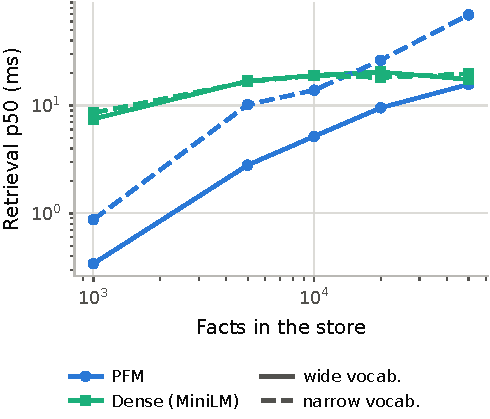
\includegraphics[width=0.59\columnwidth]{figures/crossover.pdf}
\caption{Median retrieval latency of PFM and a MiniLM dense retriever on the same synthetic stores (100 timed queries per point after 20 warm-up queries, long-lived objects frozen). Colour is the method and the dash pattern is the term distribution. Both axes are logarithmic.}
\label{fig:crossover}
\end{figure}
\section{Additional Results}
\label{app:full}

\begin{table}[h]
\centering
\small
\setlength{\tabcolsep}{4pt}
\begin{tabular}{@{}lrrrrr@{}}
\toprule
Construction & Key prec. $\uparrow$ & Key rec. $\uparrow$ & Clean $\uparrow$ & Lost $\downarrow$ & $\Delta$ clean vs rule $\uparrow$ \\
\midrule
rule keys & 1.000 & 0.807 & \cellcolor{cPos!60}0.781 & \cellcolor{cPos!60}0.047 & -- \\
\quad model keys, llama3.2:3b & 0.930 & 0.994 & 0.592 & 0.331 & $-$0.189 {\scriptsize($-$0.241, $-$0.136)} \\
\quad model keys, qwen2:7b & 0.926 & 0.991 & 0.560 & 0.342 & $-$0.221 {\scriptsize($-$0.273, $-$0.168)} \\
\quad model keys, qwen2.5:7b & 0.990 & 0.996 & 0.644 & 0.275 & $-$0.136 {\scriptsize($-$0.186, $-$0.086)} \\
\quad model keys, qwen2.5:14b & 0.969 & 0.980 & 0.593 & 0.307 & $-$0.188 {\scriptsize($-$0.240, $-$0.134)} \\
\midrule
model updates, llama3.2:3b$^\dagger$ & -- & -- & 0.292 & 0.517 & $-$0.471 {\scriptsize($-$0.563, $-$0.379)} \\
model updates, qwen2:7b$^\dagger$ & -- & -- & 0.358 & 0.308 & $-$0.404 {\scriptsize($-$0.492, $-$0.318)} \\
model updates, qwen2.5:7b$^\dagger$ & -- & -- & 0.429 & 0.521 & $-$0.333 {\scriptsize($-$0.427, $-$0.241)} \\
model updates, qwen2.5:14b$^\dagger$ & -- & -- & 0.596 & 0.279 & $-$0.167 {\scriptsize($-$0.246, $-$0.094)} \\
keyless & -- & -- & 0.243 & 0.047 & $-$0.537 {\scriptsize($-$0.590, $-$0.488)} \\
\bottomrule
\end{tabular}
\caption{Key recall does not order the construction paths; the prompt does. 720 queries over seeds 7, 11 and 13 of the rewritten corpus; one rewriter (qwen2:7b) produces the text for every arm, so the arms differ only in who assigns the keys. \emph{Key prec.} and \emph{key rec.} score the assigned keys against the generator's (entity, slot) keys, pooled over seeds, counting a misfiled key as a false positive and a missing one as a false negative; the error counts behind them are in Table~\ref{tab:key_errors}. \emph{Clean} reads as in Table~\ref{tab:temporal}. \emph{Lost}: the share of queries whose current value is in no active fact --- deleted by a false merge, which the prompt cannot show. $\Delta$: the paired difference in clean from the rule extractor on the same queries, with a chain-cluster bootstrap 95\% interval; negative means worse than the rule. $^\dagger$The Mem0-shaped path is a contrast rather than the claim under test and runs at seed 7 only, so its interval resamples that seed's chains. Shaded: the rule extractor, lowest in key recall, leaves the cleanest prompt and loses the fewest current values.}
\label{tab:extractor}
\end{table}

\begin{table}[h]
\centering
\small
\setlength{\tabcolsep}{4pt}
\begin{tabular}{@{}lrrrrl@{}}
\toprule
Key assigner & Correct $\uparrow$ & Missed $\downarrow$ & Wrong slot $\downarrow$ & Wrong entity $\downarrow$ & Commonest confusion \\
\midrule
rule keys & 1{,}023 & 245 & \cellcolor{cPos!60}0 & 0 & -- \\
llama3.2:3b & 1{,}173 & 7 & 88 & 0 & room $\to$ meeting (76) \\
qwen2:7b & 1{,}164 & 11 & 93 & 0 & room $\to$ meeting (74) \\
qwen2.5:7b & 1{,}250 & 5 & 13 & 0 & deadline $\to$ meeting (12) \\
qwen2.5:14b & 1{,}205 & 25 & 38 & 0 & room $\to$ meeting (18) \\
\bottomrule
\end{tabular}
\caption{How the keys are wrong. Entries are counts, not rates: each row splits the same 1{,}268 chain messages that need a key, pooled over three seeds, by what the assigner gave --- the right key (\emph{correct}), none (\emph{missed}), the right entity with the wrong slot, or the wrong entity --- so every row sums to 1{,}268. A missed key leaves a second value active and the prompt shows it; a wrong slot merges two slots and deletes whichever value arrived first, which nothing shows. No model assigns a key to the wrong entity, and three of the four share their commonest confusion, so it belongs to a benchmark whose slot nouns overlap rather than to one model. Shaded: the rule extractor never misfiles a slot, which is why it wins while missing more.}
\label{tab:key_errors}
\end{table}

\begin{figure}[h]
\centering
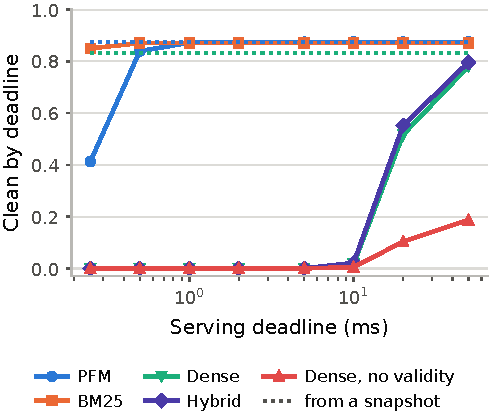
\includegraphics[width=0.59\columnwidth]{figures/deadline_curve.pdf}
\caption{Clean retrieval by deadline, $Y(D)$, on seed 7. Every arm receives $P_t$ and serves only active facts except the one marked otherwise. Solid lines: fresh retrieval, counting a run as successful only if it is clean and finishes within $D$; the four validity-restricted arms coincide above 1~ms, and Dense sits under Hybrid. Dotted: the same ranking served from a snapshot built after the latest revision, whose read takes about 1~$\mu$s; Appendix~\ref{app:serving} shows what happens when the snapshot is older.}
\label{fig:deadline}
\end{figure}

\begin{table}[h]
\centering
\scriptsize
\setlength{\tabcolsep}{3pt}
\begin{tabular}{@{}lrrrrrr@{}}
\toprule
Method & Clean & Current & Stale & Wrong & p50 (ms) & p99 (ms) \\
\midrule
PFM & 0.877 {\scriptsize(0.850, 0.904)} & 0.998 & 0.000 & 0.121 & 0.25 & 0.69 \\
BM25 + validity & 0.774 {\scriptsize(0.737, 0.809)} & 0.891 & 0.000 & 0.120 & 0.09 & 0.26 \\
BM25 + validity ($+P_t$) & 0.873 {\scriptsize(0.847, 0.896)} & 1.000 & 0.000 & 0.128 & 0.10 & 0.29 \\
Dense + validity & 0.834 {\scriptsize(0.802, 0.866)} & 0.998 & 0.000 & 0.165 & 17.9 & 88.5 \\
Dense + validity ($+P_t$) & 0.836 {\scriptsize(0.803, 0.868)} & 1.000 & 0.000 & 0.164 & 18.3 & 93.0 \\
Hybrid + validity & 0.807 {\scriptsize(0.773, 0.842)} & 0.949 & 0.000 & 0.151 & 17.5 & 79.7 \\
Hybrid + validity ($+P_t$) & 0.843 {\scriptsize(0.813, 0.872)} & 1.000 & 0.000 & 0.157 & 18.2 & 82.4 \\
\midrule
BM25 & 0.155 {\scriptsize(0.126, 0.186)} & 0.852 & 0.715 & 0.074 & 0.15 & 0.38 \\
BM25 ($+P_t$) & 0.195 {\scriptsize(0.164, 0.227)} & 0.997 & 0.802 & 0.007 & 0.18 & 0.46 \\
BM25 + recency & 0.185 {\scriptsize(0.154, 0.215)} & 0.877 & 0.667 & 0.102 & 0.18 & 0.55 \\
BM25 + recency ($+P_t$) & 0.193 {\scriptsize(0.162, 0.226)} & 0.989 & 0.784 & 0.038 & 0.21 & 0.60 \\
Dense (MiniLM) & 0.167 {\scriptsize(0.137, 0.198)} & 0.968 & 0.800 & 0.131 & 18.5 & 86.6 \\
Dense (MiniLM) ($+P_t$) & 0.181 {\scriptsize(0.151, 0.212)} & 0.989 & 0.802 & 0.060 & 19.0 & 97.4 \\
Hybrid (RRF) & 0.165 {\scriptsize(0.136, 0.195)} & 0.889 & 0.787 & 0.098 & 18.8 & 88.5 \\
Hybrid (RRF) ($+P_t$) & 0.188 {\scriptsize(0.157, 0.219)} & 0.998 & 0.802 & 0.027 & 19.0 & 96.4 \\
\bottomrule
\end{tabular}
\caption{All retrieval arms (1{,}200 queries; latency from seed 7). Clean intervals are two-level (seed, chain) bootstrap 95\% intervals.}
\label{tab:full}
\end{table}

\begin{table}[h]
\centering
\scriptsize
\setlength{\tabcolsep}{4pt}
\begin{tabular}{@{}lrrrrrrr@{}}
\toprule
Variant & Clean & $\Delta$ & Current & Stale & Wrong & Amb. clean & Amb. wrong \\
\midrule
full & 0.877 {\scriptsize(0.850, 0.904)} & +0.000 & 0.998 & 0.000 & 0.121 & 0.341 & 0.650 \\
no participant field & 0.842 {\scriptsize(0.813, 0.870)} & -0.036 & 0.996 & 0.000 & 0.154 & 0.170 & 0.830 \\
no participant terms & 0.811 {\scriptsize(0.775, 0.845)} & -0.067 & 0.943 & 0.000 & 0.133 & 0.211 & 0.717 \\
no participant seeds & 0.877 {\scriptsize(0.850, 0.904)} & +0.000 & 0.998 & 0.000 & 0.121 & 0.341 & 0.650 \\
no participants at all & 0.756 {\scriptsize(0.723, 0.788)} & -0.122 & 0.890 & 0.000 & 0.138 & 0.130 & 0.744 \\
no entity field & 0.884 {\scriptsize(0.857, 0.910)} & +0.007 & 0.998 & 0.000 & 0.114 & 0.377 & 0.614 \\
no graph & 0.877 {\scriptsize(0.850, 0.904)} & +0.000 & 0.998 & 0.000 & 0.121 & 0.341 & 0.650 \\
no usage & 0.877 {\scriptsize(0.850, 0.904)} & +0.000 & 0.998 & 0.000 & 0.121 & 0.341 & 0.650 \\
no recency & 0.879 {\scriptsize(0.854, 0.903)} & +0.002 & 1.000 & 0.000 & 0.121 & 0.350 & 0.650 \\
no positional decay & 0.871 {\scriptsize(0.843, 0.899)} & -0.007 & 0.998 & 0.000 & 0.128 & 0.305 & 0.686 \\
no term cap & 0.877 {\scriptsize(0.850, 0.904)} & +0.000 & 0.998 & 0.000 & 0.121 & 0.341 & 0.650 \\
no usage inheritance & 0.877 {\scriptsize(0.850, 0.904)} & +0.000 & 0.998 & 0.000 & 0.121 & 0.341 & 0.650 \\
text only dedup & 0.877 {\scriptsize(0.850, 0.904)} & +0.000 & 0.998 & 0.000 & 0.121 & 0.341 & 0.650 \\
no keys & 0.247 {\scriptsize(0.210, 0.284)} & -0.631 & 0.950 & 0.703 & 0.004 & 0.247 & 0.022 \\
pfm | participant filter & 0.998 {\scriptsize(0.993, 1.000)} & +0.121 & 0.998 & 0.000 & 0.000 & 0.991 & 0.000 \\
bm25 validity+P | participant filter & 1.000 {\scriptsize(0.995, 1.000)} & +0.123 & 1.000 & 0.000 & 0.000 & 1.000 & 0.000 \\
pfm | cutoff@0.5 & 0.898 {\scriptsize(0.873, 0.921)} & +0.021 & 0.998 & 0.000 & 0.100 & 0.453 & 0.538 \\
pfm | cutoff@0.7 & 0.983 {\scriptsize(0.973, 0.993)} & +0.106 & 0.992 & 0.000 & 0.008 & 0.933 & 0.045 \\
pfm | cutoff@0.9 & 0.866 {\scriptsize(0.835, 0.893)} & -0.012 & 0.866 & 0.000 & 0.000 & 0.839 & 0.000 \\
\bottomrule
\end{tabular}
\caption{Leave-one-out ablation and identity baselines (1{,}200 queries; stale exposure is zero in every keyed row). $\Delta$ is the paired difference from full PFM with a chain-bootstrap interval. $^\dagger$Each removed separately ($\gamma=0$, $\eta=0$, no term cap, no participant seeds, and also no usage inheritance or text-only deduplication); none changes the outcome of any of the 1{,}200 queries. Relative cutoff drops facts scoring below the stated fraction of the top score.}
\label{tab:ablation}
\end{table}

\begin{table}[h]
\centering
\small
\begin{tabular}{@{}lrrrrrrr@{}}
\toprule
Method & $d{=}0$ & $d{=}1$ & $d{=}2$ & $d{=}3$ & $d{=}4$ & Benchmark mix & Reweighted \\
\midrule
PFM (keyed) & 0.878 & 0.867 & 0.874 & 0.887 & 0.902 & 0.877 & 0.877 \\
PFM, keyless & 0.794 & 0.233 & 0.047 & 0.033 & 0.023 & 0.247 & 0.603 \\
BM25 + validity ($+P_t$) & 0.857 & 0.878 & 0.868 & 0.861 & 0.910 & 0.873 & 0.863 \\
Dense + validity ($+P_t$) & 0.819 & 0.850 & 0.818 & 0.848 & 0.857 & 0.836 & 0.826 \\
BM25 ($+P_t$) & 0.983 & 0.000 & 0.000 & 0.000 & 0.000 & 0.195 & 0.688 \\
\bottomrule
\end{tabular}
\caption{Clean retrieval by revision depth $d$, and aggregates under the benchmark's own mix of depths and under a store where 70\% of facts are never revised ($d$ weights 0.70, 0.18, 0.07, 0.03, 0.02).}
\label{tab:depth}
\end{table}

\begin{table}[h]
\centering
\small
\begin{tabular}{@{}lrrrrrr@{}}
\toprule
Method & seed 7 & seed 11 & seed 13 & seed 17 & seed 19 & Mean $\pm$ sd \\
\midrule
PFM & 0.875 & 0.912 & 0.875 & 0.854 & 0.871 & 0.877 $\pm$ 0.021 \\
BM25 + validity & 0.754 & 0.812 & 0.754 & 0.783 & 0.767 & 0.774 $\pm$ 0.025 \\
BM25 + validity ($+P_t$) & 0.871 & 0.892 & 0.867 & 0.867 & 0.867 & 0.873 $\pm$ 0.011 \\
Dense + validity ($+P_t$) & 0.833 & 0.867 & 0.812 & 0.850 & 0.817 & 0.836 $\pm$ 0.023 \\
Hybrid + validity ($+P_t$) & 0.842 & 0.863 & 0.829 & 0.858 & 0.825 & 0.843 $\pm$ 0.017 \\
BM25 ($+P_t$) & 0.212 & 0.179 & 0.208 & 0.183 & 0.192 & 0.195 $\pm$ 0.015 \\
Dense (MiniLM) ($+P_t$) & 0.200 & 0.167 & 0.179 & 0.171 & 0.188 & 0.181 $\pm$ 0.013 \\
\bottomrule
\end{tabular}
\caption{Clean retrieval per benchmark seed (240 queries each).}
\label{tab:seeds}
\end{table}

\begin{figure}[h]
\centering
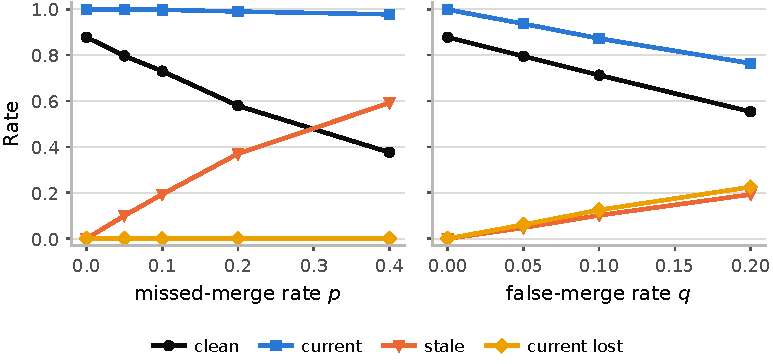
\includegraphics[width=0.94\columnwidth]{figures/keynoise.pdf}
\caption{Keyed PFM under injected key errors (1{,}200 queries). Left: missed merges at rate $p$ ($q=0$). Right: false merges at rate $q$ ($p=0$). ``Current lost'': the current value is held by no active fact, which is the failure the prompt does not show. Table~\ref{tab:keynoise} gives the full $p\times q$ grid.}
\label{fig:keynoise}
\end{figure}

\begin{table}[h]
\centering
\scriptsize
\begin{tabular}{@{}lcccc@{}}
\toprule
$p$ (rows), $q$ (columns) & 0 & 0.05 & 0.1 & 0.2 \\
\midrule
0 & 0.877 / 0.000 / 0.000 & 0.795 / 0.048 / 0.061 & 0.713 / 0.102 / 0.125 & 0.553 / 0.193 / 0.225 \\
0.05 & 0.797 / 0.100 / 0.000 & 0.709 / 0.152 / 0.068 & 0.614 / 0.210 / 0.129 & 0.496 / 0.271 / 0.214 \\
0.1 & 0.730 / 0.193 / 0.000 & 0.637 / 0.242 / 0.062 & 0.562 / 0.281 / 0.118 & 0.460 / 0.332 / 0.205 \\
0.2 & 0.579 / 0.370 / 0.000 & 0.522 / 0.398 / 0.048 & 0.462 / 0.425 / 0.102 & 0.368 / 0.463 / 0.186 \\
0.4 & 0.376 / 0.592 / 0.000 & 0.341 / 0.592 / 0.044 & 0.331 / 0.587 / 0.083 & 0.288 / 0.598 / 0.121 \\
\bottomrule
\end{tabular}
\caption{Key-noise grid: clean retrieval / stale exposure / share of queries whose current value is not active (1{,}200 queries per cell).}
\label{tab:keynoise}
\end{table}

\section{Misattribution and Abstention on LoCoMo}
\label{app:locomo}

\paragraph{Misattribution is worse on real text, and nothing we have removes it.} Over one store built from all ten conversations (13{,}435 facts, 537 questions, 186 of them from the three conversations with a name-sharing speaker), more than half the prompts for a question about such a speaker carry a fact from another one's conversation, judged by provenance rather than by any value label: 0.543, with 37\% of all served lines coming from a conversation other than the question's own. Filtering on the interlocutor halves that to 0.301 and here costs no recall, because LoCoMo's questions are about the speakers themselves. The graph affinity of Section~\ref{sec:identity} cuts off-conversation lines from 0.371 to 0.237 and leaves exposure where it was (Table~\ref{tab:locomo}).

The posterior of Eq.~(\ref{eq:identity}) does not apply at all, for a reason worth stating plainly: it chooses between distinct stored entities, which works when the store holds ``Alex Chen'' and ``Alex Rivera'', and LoCoMo's two Johns are both the string \texttt{john}. There is no surface form to choose between, so the posterior is empty and the ranking untouched; the only evidence separating them is who each is discussed with, which the affinity term uses and which is not enough. The exposure our benchmark puts at 0.121 and our posterior at 0.032 is 0.543 here and stays there. Identity is the axis of the three we leave open.

\paragraph{Abstention on an open corpus costs more than it saves.} Rebuilding one store per conversation and asking each both its own 537 questions and 1{,}800 questions borrowed from the other nine, the ungated ranker returns a block for almost every request it cannot answer (it abstains on 7.3\%, when nothing scores at all). The margin gate does abstain, on 95.0\% of the unanswerable requests at $\tau=1.5$, but it also abstains on 73.9\% of the answerable ones and drops current-value recall from 0.220 to 0.099, and raising $\tau$ only moves further along the same curve (0.964 and 0.870 at $\tau=2$, 0.983 and 0.968 at $\tau=3$). No operating point on this corpus buys abstention at a recall cost worth paying. The slot gate, which does buy it on our benchmark for 0.002, cannot run here at all: it needs an inventory of slots, and this corpus has none. Abstention is therefore solved when the schema is known and unsolved when it is not.

\begin{table}[h]
\centering
\small
\setlength{\tabcolsep}{4pt}
\begin{tabular}{@{}lrrrr@{}}
\toprule
Serving rule & Wrong person & \quad name-sharing & Off-conversation lines & Current \\
\midrule
none & 0.188 & 0.543 & 0.371 & 0.078 \\
participant filter & 0.104 & 0.301 & 0.087 & 0.102 \\
context affinity & 0.190 & 0.548 & 0.237 & 0.050 \\
\bottomrule
\end{tabular}
\caption{Misattribution on LoCoMo, judged by provenance over one store built from all ten conversations (13{,}435 facts, 537 questions, of which 186 come from the three conversations with a name-sharing speaker). ``Wrong person'': the block holds a fact from a conversation whose speakers share the queried first name. ``Off-conversation lines'': the share of all served lines that come from another conversation. ``Current'': the gold answer occurs in the block, which lexical retrieval over sentence-level facts achieves rarely on this corpus, so the column bounds exposure and not recall.}
\label{tab:locomo}
\end{table}
\section{Query-Time Model Baselines}
\label{app:systems}\label{sec:systems}

Each of the three failures can also be attacked by a model call on the request path, which is what a memory that keeps every version and resolves conflicts on read must do. We put three such baselines on the same corpora, arms and metrics as the rules they would replace (480 main-benchmark queries over two seeds, 180 hard-slice queries; Table~\ref{tab:systems}). A \emph{temporal reranker} sees the dated candidate lines of a validity-agnostic retriever and names the ones in force. An \emph{entity resolver} sees the request and the people its name could denote and picks one. An \emph{abstention judge} sees the block and the request and says whether the block answers it.

The reranker recovers less than half of what write-time supersession gives and pays for it twice. It does cut stale exposure, from 0.800 to 0.381, but current-value recall falls from 0.998 to 0.454 as it discards lines it should have kept, so clean retrieval reaches 0.302 against the keyed store's 0.894 --- and it costs 654~ms at the median on the request path, against 0.25~ms for the whole lexical retrieval it is reranking. The abstention judge is worse: it abstains on two thirds of the unanswerable hard-slice requests, where the slot gate abstains on all of them, and abstains so freely elsewhere that clean retrieval falls from 0.894 to 0.569, for 912~ms a request.

Entity resolution is the one place the model call is competitive. It cuts wrong-person exposure from 0.106 to 0.031 and reaches 0.931 clean, which is what the posterior of Eq.~(\ref{eq:identity}) reaches at 0.969 for no model call at all, and it fires only on ambiguous mentions, so its median request-path cost is zero and its 99th percentile is 1{,}967~ms. The pattern across the three is the same: where a cheap rule exists the model call matches it at a thousand times the latency, and where no cheap rule exists the model call does not supply one either.

\begin{table}[h]
\centering
\small
\setlength{\tabcolsep}{4pt}
\begin{tabular}{@{}lrrrrr@{}}
\toprule
Arm & Stale & Wrong & Clean & Abstained (no answer) & Model ms p50 \\
\midrule
bm25+P & 0.800 & 0.006 & 0.196 & 0.000 & -- \\
llm temporal rerank & 0.381 & 0.008 & 0.302 & 0.000 & 653.6 \\
pfm & 0.000 & 0.106 & 0.894 & 0.000 & -- \\
identity hard & 0.000 & 0.031 & 0.969 & 0.000 & -- \\
identity hard|abstain slot@0.5 & 0.000 & 0.031 & 0.969 & 1.000 & -- \\
llm abstain & 0.000 & 0.054 & 0.569 & 0.667 & 912.1 \\
llm entity resolve & 0.000 & 0.031 & 0.931 & 0.000 & 0.01 \\
participant filter & 0.000 & 0.000 & 1.000 & 0.000 & -- \\
\bottomrule
\end{tabular}
\caption{Query-time model calls against the serving-side rules they would replace (qwen2:7b; 480 main-benchmark queries over seeds 7 and 11, 180 hard-slice queries). Stale, wrong and clean are on the main benchmark; ``abstained'' is on the 60 unanswerable hard-slice requests. ``Model ms'' is the median wall time of the request-path model call, which is zero for the entity resolver because it fires only on an ambiguous mention (its 99th percentile is 1{,}967~ms). The reranker is applied to BM25 + $P_t$, which is the arm that needs it; every other row serves active facts.}
\label{tab:systems}
\end{table}

\section{Response Level}
\label{app:llm}

Table~\ref{tab:llm} reports the 7B model on the main benchmark and Table~\ref{tab:llm_llama} the 3B model on the same blocks. Two further studies check that those conclusions do not rest on an unbroken prompt or on greedy decoding.

\paragraph{Conditions that break the prompt.} We repeat the measurement where the store is wrong rather than right. Under injected key noise at $p=q=0.05$ the block carries a superseded value on 18.3\% of requests, and the models write one on 4.2\% (7B) and 10.0\% (3B), so a prompt-level error rate again overstates what reaches the text, and again by less for the smaller model. Out-of-order arrival is the harder case: the block carries a superseded value on 13.3\% of requests and the 7B model writes one on 13.3\%, repeating essentially everything it is shown. We read the difference as a property of what the stale value looks like --- a key-noise prompt usually holds the current value beside the stale one, an out-of-order prompt often holds the stale one alone --- and not as a property of the models.

On the hard-identity slice the serving rules of Section~\ref{sec:identity} carry into the text. With no rule the block holds a competitor's value on every request and the models write it on 30.6\% and 33.3\%. The identity posterior removes the exposure on the answerable requests, leaving it only on the unanswerable ones, and the completion rate does not move (0.333 and 0.306), because the requests it still exposes are exactly the ones the models answer wrongly. Adding the slot gate removes both: 100\% of the 7B model's completions and 97.2\% of the 3B model's are correct, where correct on an unanswerable request means naming no value.

\paragraph{Sampling rather than greedy decoding.} We repeat the keyed-versus-keyless comparison at temperature 0.7 with three decoding seeds, 720 completions per arm. The keyed store reaches 0.921 correct against 0.929 greedy, and the keyless store 0.692 against 0.704, so the gap is 0.229 sampled against 0.225 greedy. The comparison does not depend on the decoding rule.

\begin{table}[h]
\centering
\footnotesize
\setlength{\tabcolsep}{3.5pt}
\begin{tabular}{@{}lrrrrrrrrrr@{}}
\toprule
Memory & Curr. & Stale & Wrong & Correct & Mixed & Stale & Wrong & Other & Chars & TTFT \\
\midrule
None & -- & -- & -- & 0.000 & 0.000 & 0.004 & 0.000 & 0.996 & 0 & 325 \\
PFM & 1.000 & 0.000 & 0.125 & 0.929 & 0.000 & 0.000 & 0.013 & 0.058 & 472 & 1229 \\
PFM, keyless & 0.908 & 0.642 & 0.013 & 0.704 & 0.008 & 0.188 & 0.000 & 0.100 & 476 & 1236 \\
BM25 & 0.854 & 0.692 & 0.092 & 0.629 & 0.000 & 0.254 & 0.004 & 0.113 & 468 & 1365 \\
BM25 + latest-value instruction & 0.854 & 0.692 & 0.092 & 0.654 & 0.000 & 0.233 & 0.004 & 0.108 & 468 & 1506 \\
BM25 + validity & 0.887 & 0.000 & 0.133 & 0.842 & 0.000 & 0.000 & 0.004 & 0.154 & 465 & 1388 \\
Dense + validity & 1.000 & 0.000 & 0.171 & 0.946 & 0.000 & 0.000 & 0.000 & 0.054 & 476 & 1469 \\
\bottomrule
\end{tabular}
\caption{Response level on the 240 seed-7 queries (qwen2:7b, greedy). Prompt columns: exposure in the injected block. Completion columns: judged outcome. Chars: mean block length. TTFT: median time to first token in ms, including a full prefill. The ``None'' arm has no memory, so its zero correct rate holds by construction.}
\label{tab:llm}
\end{table}
\begin{table}[h]
\centering
\footnotesize
\setlength{\tabcolsep}{3.5pt}
\begin{tabular}{@{}lrrrrrrrrrr@{}}
\toprule
Memory & Curr. & Stale & Wrong & Correct & Mixed & Stale & Wrong & Other & Chars & TTFT \\
\midrule
None & -- & -- & -- & 0.000 & 0.000 & 0.000 & 0.000 & 1.000 & 0 & 168 \\
PFM & 1.000 & 0.000 & 0.125 & 0.912 & 0.000 & 0.000 & 0.017 & 0.071 & 472 & 544 \\
PFM, keyless & 0.908 & 0.642 & 0.013 & 0.592 & 0.000 & 0.279 & 0.000 & 0.129 & 476 & 623 \\
BM25 & 0.854 & 0.692 & 0.092 & 0.454 & 0.000 & 0.408 & 0.004 & 0.133 & 468 & 830 \\
BM25 + latest-value instruction & 0.854 & 0.692 & 0.092 & 0.504 & 0.000 & 0.321 & 0.004 & 0.171 & 468 & 648 \\
BM25 + validity & 0.887 & 0.000 & 0.133 & 0.817 & 0.000 & 0.000 & 0.004 & 0.179 & 465 & 809 \\
Dense + validity & 1.000 & 0.000 & 0.171 & 0.887 & 0.000 & 0.000 & 0.008 & 0.104 & 476 & 829 \\
\bottomrule
\end{tabular}
\caption{Response level with the second model (llama3.2:3b, 4-bit, greedy) on the same 240 queries and the same blocks as Table~\ref{tab:llm}.}
\label{tab:llm_llama}
\end{table}
\begin{table}[h]
\centering
\scriptsize
\setlength{\tabcolsep}{3.5pt}
\begin{tabular}{@{}lllrrrrrr@{}}
\toprule
Condition & Model & Memory & $n$ & Prompt stale & Prompt wrong & Correct & Stale & Wrong \\
\midrule
hard identity & llama3.2 & PFM & 36 & 0.000 & 1.000 & 0.694 & 0.000 & 0.306 \\
hard identity & llama3.2 & pfm identity & 36 & 0.000 & 0.333 & 0.694 & 0.000 & 0.306 \\
hard identity & llama3.2 & pfm identity abstain & 36 & 0.000 & 0.000 & 0.972 & 0.000 & 0.000 \\
hard identity & qwen2 & PFM & 36 & 0.000 & 1.000 & 0.667 & 0.000 & 0.333 \\
hard identity & qwen2 & pfm identity & 36 & 0.000 & 0.333 & 0.667 & 0.000 & 0.333 \\
hard identity & qwen2 & pfm identity abstain & 36 & 0.000 & 0.000 & 1.000 & 0.000 & 0.000 \\
key noise p=0.05 q=0.05 & llama3.2 & PFM & 240 & 0.183 & 0.087 & 0.754 & 0.100 & 0.017 \\
key noise p=0.05 q=0.05 & qwen2 & PFM & 240 & 0.183 & 0.087 & 0.825 & 0.042 & 0.017 \\
out of order 0.3 & llama3.2 & PFM & 240 & 0.133 & 0.108 & 0.796 & 0.125 & 0.013 \\
out of order 0.3 & qwen2 & PFM & 240 & 0.133 & 0.108 & 0.804 & 0.133 & 0.008 \\
sampling & qwen2 & PFM & 720 & 0.000 & 0.125 & 0.921 & 0.000 & 0.010 \\
sampling & qwen2 & pfm keyless & 720 & 0.642 & 0.013 & 0.692 & 0.186 & 0.000 \\
\bottomrule
\end{tabular}
\caption{Response level where the prompt is broken on purpose. Prompt columns are exposure in the injected block; the last three are the judged completion. The sampling rows are 720 completions per arm at temperature 0.7 over three decoding seeds; every other row is greedy.}
\label{tab:llm_slices}
\end{table}

\section{Benchmark Slices}
\label{app:slices}\label{sec:slices}

The results so far hold on a benchmark where each slot has one value, messages arrive in the order they were written, the participant of a message is the person the fact is about, and every query has an answer. Four slices break one assumption each, with the same generator, arms and metrics (Table~\ref{tab:slices}).

Key granularity cuts both ways: when one person holds both a standup and a sync, a key at (entity, slot) merges them and current-value recall falls to 0.500, while a key at (entity, slot, noun) recalls every current value and the keyless store exposes a superseded value on every query. Coarse keys delete and fine keys stop recognizing revisions; the main benchmark hides the choice because each (entity, slot) pair has one instance. Arrival order is not statement order: delivering 30\% of chains out of order costs a transaction-time store 0.130 clean retrieval (0.877 to 0.747) with stale exposure 0.156, because a late message restating an old value closes the newer one, and Proposition~\ref{prop:one_active} still holds with the wrong value active. Ordering by stated time restores the in-order numbers exactly, at the cost of trusting a stated time at commit.

The other two slices are what Section~\ref{sec:idresults} answers. Clean retrieval holds up across subject, third-party, group and missing participants (0.865 to 0.965), because the fact text names its subject, but the hard participant filter then recalls the current value on 2.0\% of third-party facts and 1.0\% of facts with no participant: identity filtering buys exposure with recall, at a price set by how often facts concern someone other than the interlocutor. And nothing abstains. With same-first-name people whose messages share slot, noun, template and arrival day, every arm exposes the competitor's value on every query except the participant filter and a relative cutoff at 0.7 (which leaves 0.092); on queries whose answer is not in the store, every arm fills the block with someone else's value of the right type, and the cutoff does not help, because the exposure comes from the top-scoring facts.

\paragraph{Leave-one-out ablation.}\label{sec:ablation}

Removing one component at a time (Table~\ref{tab:ablation}) leaves only the participant signals with a measurable effect: dropping the participant field, the participant query terms, or both costs 0.036, 0.067 and 0.122 clean retrieval, and on ambiguous queries clean retrieval falls from 0.341 to 0.130. The entity field, the entity graph, the usage term, recency and the term cap change nothing; removing the graph or the usage term changes no query's outcome at all. We read that as a property of this benchmark rather than a general finding, and claim nothing for those components as ranking signals. Taken with the equivalence test above, what our retrieval results support is a store that serves only active facts together with participant-aware lexical retrieval. They do not support the rest of Section~\ref{sec:pfm}, and we do not ask the reader to accept it; it is described in full so the ablation has something to remove. The graph edges do earn their place, but for a decision ranking cannot make: Section~\ref{sec:idresults} uses them to choose which of two people a first name denotes.

\paragraph{Identity baselines on the main benchmark.} A hard participant filter removes all wrong-person exposure and lifts clean retrieval to 0.998; a relative score cutoff at 0.7 reaches 0.983, and at 0.9 it removes the exposure along with 13\% of current values. Both exploit a property of this benchmark, that the participant is the subject of the fact, which Section~\ref{sec:slices} removes and Section~\ref{sec:idresults} replaces with a rule that does not need it.

\begin{table}[h]
\centering
\scriptsize
\setlength{\tabcolsep}{4pt}
\begin{tabular}{@{}lrrrrr@{}}
\toprule
Condition & $n$ & Current & Stale & Wrong & Clean \\
\midrule
\emph{Two instances of one slot type} &  &  &  &  &  \\
key(entity,slot) & 240 & 0.500 & 0.000 & 0.000 & 0.500 \\
key(entity,slot,noun) & 240 & 1.000 & 0.000 & 0.000 & 1.000 \\
keyless & 240 & 1.000 & 1.000 & 0.000 & 0.000 \\
\midrule
\emph{Out-of-order arrival} &  &  &  &  &  \\
in order & 1200 & 0.998 & 0.000 & 0.121 & 0.877 \\
out of order & 1200 & 0.846 & 0.156 & 0.103 & 0.747 \\
out of order, event time & 1200 & 0.998 & 0.000 & 0.121 & 0.877 \\
\midrule
\emph{Participant is not the subject} &  &  &  &  &  \\
pfm, subject & 400 & 0.995 & 0.000 & 0.068 & 0.927 \\
pfm, third party & 200 & 0.985 & 0.000 & 0.120 & 0.865 \\
pfm, group & 400 & 0.995 & 0.000 & 0.030 & 0.965 \\
pfm, missing & 200 & 1.000 & 0.000 & 0.070 & 0.930 \\
pfm, participant filter, subject & 400 & 1.000 & 0.000 & 0.005 & 0.995 \\
pfm, participant filter, third party & 200 & 0.020 & 0.000 & 0.005 & 0.020 \\
pfm, participant filter, group & 400 & 0.998 & 0.000 & 0.000 & 0.998 \\
pfm, participant filter, missing & 200 & 0.010 & 0.000 & 0.000 & 0.010 \\
\midrule
\emph{Hard name collisions and unanswerable queries} &  &  &  &  &  \\
pfm & 120 & 1.000 & 0.000 & 1.000 & 0.000 \\
pfm, unanswerable & 60 & 0.000 & 0.000 & 1.000 & 0.000 \\
pfm, cutoff@0.7 & 120 & 1.000 & 0.000 & 0.092 & 0.908 \\
pfm, cutoff@0.7, unanswerable & 60 & 0.000 & 0.000 & 1.000 & 0.000 \\
pfm, participant filter & 120 & 1.000 & 0.000 & 0.000 & 1.000 \\
pfm, participant filter, unanswerable & 60 & 0.000 & 0.000 & 1.000 & 0.000 \\
\bottomrule
\end{tabular}
\caption{Slices that break one assumption of the main benchmark. Rows within a block share a corpus. For unanswerable queries, ``wrong'' counts blocks that contain some other person's value of the queried slot type, and ``clean'' is the second case of Eq.~(\ref{eq:clean}), which requires exposing none; no arm in this table can return an empty block, so every one of them scores zero there, and Table~\ref{tab:identity} adds the arms that can.}
\label{tab:slices}
\end{table}
\section{Proofs}
\label{app:proofs}

\subsection{Proposition~\ref{prop:one_active}}

\begin{proof}
Order the commits that carry key $\kappa$ by commit time $u_1<u_2<\cdots$. Because commits are atomic with respect to readers, every reader-visible state lies between two consecutive commits, and it suffices to show the claim after each commit. Before $u_1$ it holds by assumption. Suppose it holds before commit $j$. If no fact with key $\kappa$ is active, commit $j$ activates the new fact $f_j$ with $a_{f_j}=u_j$ and $b_{f_j}=\infty$, leaving exactly one active fact. Otherwise the induction hypothesis says the active fact $f$ with key $\kappa$ is unique, and the commit sets $b_f=u_j$ and $a_{f_j}=u_j$. Since intervals are half-open, $f$ is inactive and $f_j$ active at every $\tau\ge u_j$ until a later commit closes $f_j$, so the count stays at one. Commits for other keys and pruning (which never removes the active fact of a key) do not change activity intervals of facts with key $\kappa$. By induction the claim holds after every commit and hence in every reader-visible state.
\end{proof}

The argument uses only the commit order. If revisions arrive out of order, the invariant still holds but the surviving value is the latest to arrive.

\subsection{Proposition~\ref{prop:waiting}}

\begin{proof}
Snapshot mode. The request thread performs one reference read. By (ii) it never blocks on construction or a worker, by (v) it runs within $\sigma$ of becoming runnable, and by (iii) the read takes at most $r$; by (i) the reference always points to a complete snapshot. The added time is at most $\sigma+r$.

Fresh mode. The request thread enqueues its context, which by (iv) takes at most $h$ and does not block on the worker, then waits on a completion event with timeout $\omega_t$. If the worker finishes within $\omega_t$, the wait returns and, by (v), the request resumes at most $\sigma$ later, for at most $h+\omega_t+\sigma$. Otherwise the timeout expires, the thread sets the cancellation flag without blocking, and reads the snapshot as in snapshot mode, for a total of at most $h+\omega_t+\sigma+r$. In neither case does the request thread wait for a lock or an operation of construction, so the bounds do not depend on extraction, index maintenance, graph updates, or pruning.
\end{proof}

Two things the statement does not give. It is a bound conditional on $h$ and $\sigma$, so it is informative only with measurements of them on this path, which is what Appendix~\ref{app:serving} reports; a scheduling delay measured on some other operation of the same process does not bound $\sigma$ here, and an earlier version of this paper reported one that did not. And the worker itself may wait for the store lock, for example during a pruning pass; cancellation lets it exit as soon as it acquires the lock, so abandoned retrievals do not pile up behind construction, but a fresh request issued while the single worker is still draining a cancelled one queues behind it, and that queueing is inside $h$. The bound excludes model latency and says nothing about the age of the snapshot returned.

\end{document}
